\documentclass{scrartcl}
\usepackage[secthm]{evan}
\usepackage{asymptote}
\usepackage{mathtools}
\usepackage{enumitem}
\usepackage[document]{ragged2e}
\usepackage{graphicx}
\usepackage{wrapfig}
\usepackage{float}
\usepackage{xfrac}
\usepackage{esint}
\usepackage{footnote}
\usepackage{hyperref}
\usepackage{lipsum}
\newcommand\blfootnote[1]{
    \begingroup
    \renewcommand\thefootnote{}\footnote{#1}%
    \addtocounter{footnote}{-1}%
    \endgroup
}
\title{USAPhO for Dummies}
\author{Mayank Kumar}
\date{December 1, 2020}
\begin{document}
    \maketitle
    \section{Mechanics}
    \begin{itemize}
        \item Drag force where $C$ is the drag coefficient, $v$ is velocity, $A$ is cross-sectional area, and $\rho$ is air density is \[F_D=\frac 12C\rho Av^2\]
        \item Coriolis force (where $\omega$ is the angular velocity of the planet/disk, $v$ is the person's velocity north or south, and $\phi$ is the latitude): $\boxed{F=2m\omega v\sin\phi}$ Note that $\phi$ is also the angle between $\omega$ and $v$, thus, more generally, \[\vec{\mathbf F}_\text{Coriolis}=2m\vec{\mathbf \omega}\times\vec{\mathbf v}\] If it's a disk, then $\phi=\pi/2$ and $v$ is just the radial velocity of an object.
        \item More generally, whenever trying to convert from an inertial frame of reference to one that is rotating with angular velocity $\omega$, there are three pseudo-forces to consider: the Euler force (which is the tangential force cause by variable $\omega$), the Coriolis force, and the centrifugal force. The general equation is, \[\vec{\mathbf F}_K-m\dot{\mathbf{\omega}}\times\vec{\mathbf r}_{K'}-2m\vec{\mathbf \omega}\times\vec{\mathbf v}_{K'}-m\vec{\mathbf \omega}\times\left(\vec{\mathbf \omega}\times\vec{\mathbf r}_{K'}\right)=m\vec{\mathbf a}_{K'}\]
        \item Tension in a ring of radius $r$ rotating at $\omega$ (note to find tension, just divide scalar sum of force by circumference): \[T=\frac{m\omega^2 r}{2\pi}\]
        \item Radius of curvature ($R_C$) of a body's trajectory (given by the function $y(x)$) is \[R_C=\left|\frac{\left[1+\left(y'\right)^2\right]^{\frac32}}{y''}\right|\]
        \item A force $\vec{\mathbf F}=F_x\mathbf{\hat i}+F_y\mathbf{\hat j}+F_z\mathbf{\hat k}$  is conservative if and only if
        \[\vec{\mathbf \nabla}\times\vec{\mathbf F}=\begin{vmatrix}
            \mathbf{\hat i} & \mathbf{\hat j} & \mathbf{\hat k} \\
            \\\dfrac{\partial}{\partial x} & \dfrac{\partial}{\partial y} & \dfrac{\partial}{\partial z}\\
            \\F_x & F_y & F_z \\
        \end{vmatrix}=0\]
        \item A force is central if and only if $\vec{\mathbf r}\times\vec{\mathbf F}=0$ everywhere where $\vec{\mathbf r}$ is the position vector of a point from the ``center." So, a force cannot produce a net torque on a particle, anywhere in its field.
        \item If $\vec{{\mathbf A}}$ is the area sweeped by a body of mass $m$, then the angular momentum is $\vec{\mathbf L}=2m\dot{\mathbf A}$
        \item If an object is in unstable equilibrium, then the graph of potential energy vs. position will have a local maxima. A local minima will occur at stable equilibrium, and $U''=0$ at neutral equilibrium, i.e. the graph is constant.
        \item Potential energy for an object moving under the influence of  force $\vec{\mathbf F}$ is given by \[\Delta U=-\int \vec{\mathbf F}\cdot\mathrm d\vec{\mathbf s}\implies\vec{\mathbf F}=-\frac{\partial U}{\partial x}\mathbf{\hat i}-\frac{\partial U}{\partial y}\mathbf{\hat j}-\frac{\partial U}{\partial z}\mathbf{\hat k}=-\vec\nabla U\] Here, the del operator ($\vec\nabla$) denotes ``gradient." It can also denote the divergence or curl (both of which are advanced topic, don't worry). Anyway, here $U$ is a scalar field whose function is given in rectangular co-ordinates. The above formula for $\vec\nabla$ is valid only for this co-ordinate system. For spherical co-ordinates, this changes to \[\vec\nabla=\frac{\partial\hat{\mathbf r}}{\partial r}+\frac1r\frac{\partial\hat{\mathbf{\theta}}}{\partial \theta}+\frac1{r\sin\theta}\frac{\partial\hat{\mathbf{\varphi}}}{\partial\varphi}\] and in cylindrical co-ordinates it's, \[\vec\nabla=\frac{\partial\hat{\mathbf{\rho}}}{\partial\rho}+\frac1\rho\frac{\partial\hat{\mathbf{\varphi}}}{\partial\varphi}+\frac{\partial\hat{\mathbf z}}{\partial z}\]
        \begin{figure}[H]
            \centering
            \begin{minipage}[b]{0.4\textwidth}
                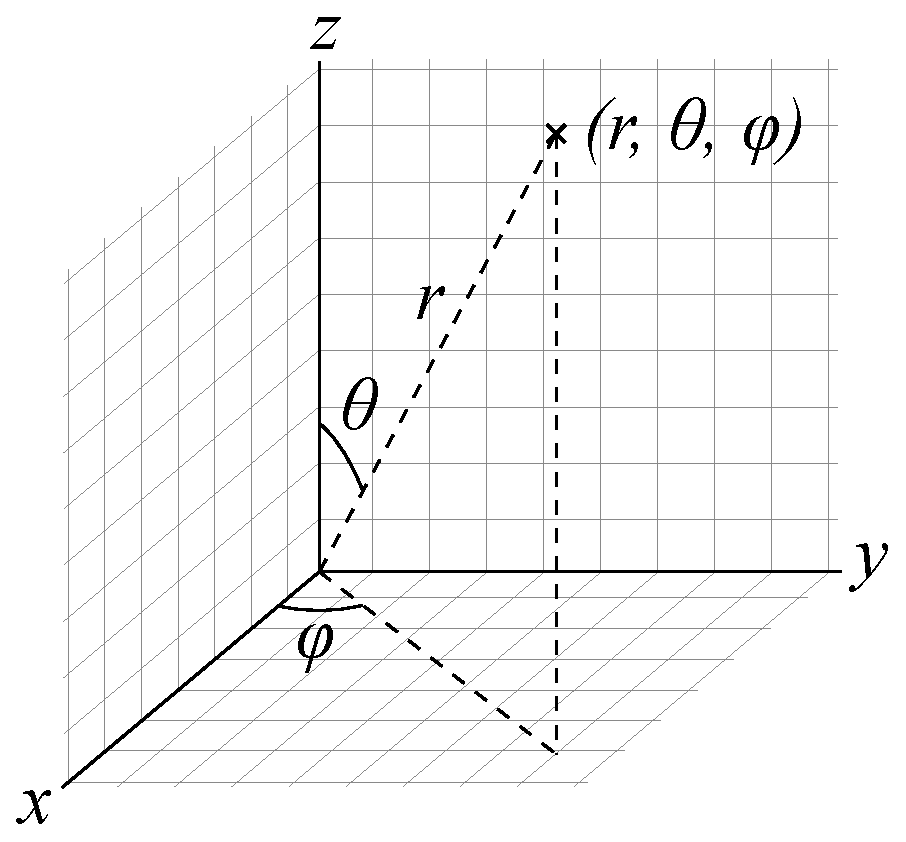
\includegraphics[width=\textwidth]{sphere.eps}
                \caption{Spherical co-ordinates.}
            \end{minipage}
            \hfill
            \begin{minipage}[b]{0.4\textwidth}
                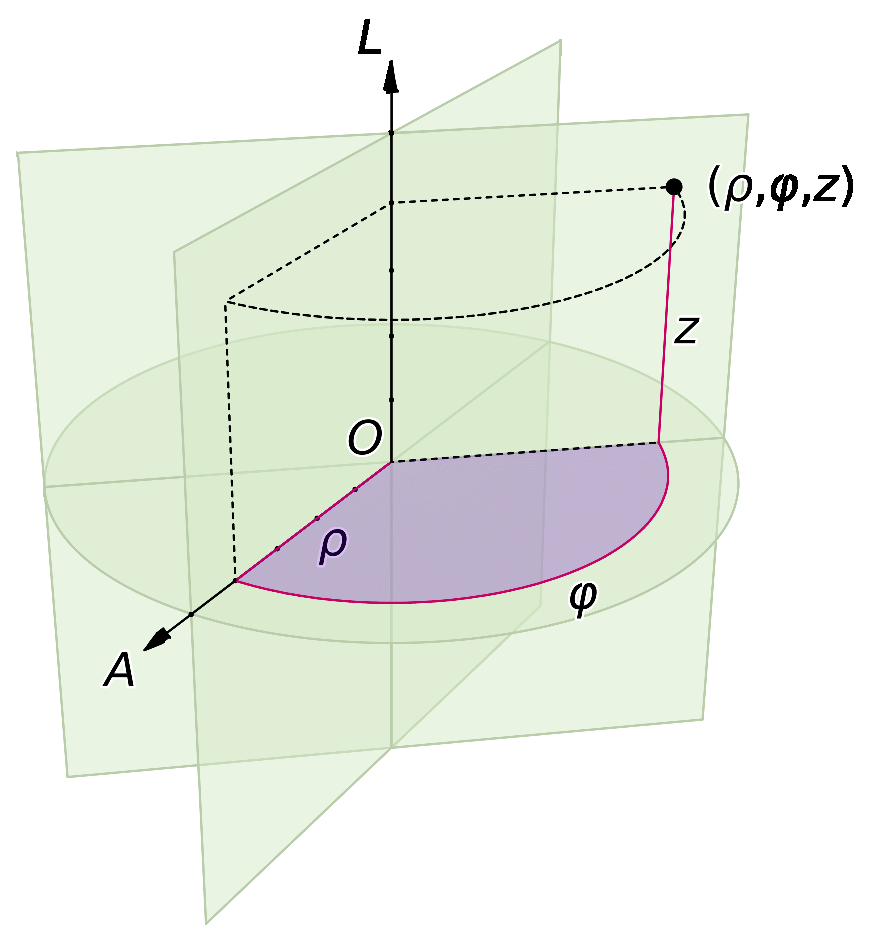
\includegraphics[width=\textwidth]{cylinder.eps}
                \caption{Cylindrical co-ordinates.}
            \end{minipage}
        \end{figure}
        \item If 2 objects have a perfectly elastic collision, then their velocities are given by \[v_1=\frac{m_1-m_2}{m_1+m_2}u_1+\frac{2m_2}{m_1+m_2}u_2\]\[v_2=\frac{2m_1}{m_1+m_2}u_1-\frac{m_1-m_2}{m_1+m_2}u_2\] where $m_1$ and $m_2$ are their respective masses and $u_1$ and $u_2$ are their respective initial velocities.
        \item To find the distance from center ($x$) where a force has more torque than linear force, use the equation $I=mxR$.
        \item For bodies rolling from a height $h$ on a ramp inclined at $\theta$ from the horizontal, the velocity at the bottom is \[v_\text{bot}=\sqrt{\frac{2gh}\beta}\] the acceleration is \[a=\frac{g\sin\theta}\beta\] and the time it takes for the object to reach the bottom is \[t=\sqrt{\frac{2h\beta}{g\sin^2\theta}}\] where \[\beta=1+\frac I{mR^2}\]
        \item To shift the position of normal force $x$  to the right, apply \[F=\frac{mgh}x\] at a height $h$. To topple the box, let $x=b/2$ where $b$ is the width of the box.
        \item Definition of simple harmonic motion is if a body's motion satisfies the equation $m\ddot x+C_0x=0$. Solving it, we get \[x=x_0\sin(\omega t+\phi)\] where $\omega^2=C_0/M$. Here $\omega$ is the angular frequency of oscillation and not angular velocity.
        \item Time period is given by \[T=\frac{2\pi}\omega=2\pi\sqrt{\frac M{C_0}}=\nu^{-1}\] The velocity at any point $x$ is given by\[v=\omega\sqrt{A^2-x^2}\]
        \item The potential and kinetic energy of the object is given respectively by \[U=\frac12m\omega^2x^2=\frac12C_0x^2\]\[K=\frac12m\omega^2(A^2-x^2)=\frac12C_0(A^2-x^2)\]
        \item For any pendulum, the time period is \[T=2\pi\sqrt{\frac I{mxa}}\] where $a$ is the downward acceleration (in most cases it is $g$) and $x$= distance between pivot and C.O.M.
        \item For a torsion pendulum, the equation is \[T=2\pi\sqrt{\frac I\kappa}\] where $I$ is the moment of inertia about axis of rotation and $\kappa$ is the torsion constant.
        \item The angular velocity of the shaft of length $L$  of a precessing  gyroscope of mass $M$, moment of inertia $I$, and angular velocity $\omega$: \[\Omega=\frac{MgL}{I\omega}\]
    \end{itemize}
    \section{Gravitation}
    \begin{itemize}
        \item Gravitational field intensity at a point is the gravitational force on a unit mass at that point, i.e. \[\frac{GM}{r^2}\]
        \item For a body orbiting a much more massive body (of mass $M$) the Vis-Visa Equation says \[v^2=GM\left(\frac2r-\frac1a\right)\] where $v$  is relative velocity, $r$ is the distance between the bodies, and $a$ is the semi-major axis of the orbit. For elliptical, circular, parabolic, and hyperbolic orbits, $a>0$, $a=0$, $a=\infty$, and $a<0$, respectively. The total angular momentum of the orbiting body is given by \[L=mb\sqrt{\frac{GM}a}\]  where $b$  is the semi-minor axis.
    \end{itemize}
    \section{Bulk Matter}
    \begin{itemize}
        \item Stress is defined as the force applied per unit area (units are Pa) and strain is deformation. Young's modulus is given by \[Y=\frac{\text{longitudinal/parallel stress}}{\text{linear strain}}=\frac{F/A_\text{cross}}{\Delta L/L_0}=\frac{FL_0}{A_\text{cross}\Delta L}\]
        \item Bulk modulus is the effect of pressure on volume; it's mainly used for gases. Solids have  very low $B$ and for ideal liquids, $B=0$. It is defined as \[B=\frac1C=\frac{\text{compressive/normal stress}}{\text{volumetric strain}}=-\frac{F/A_\text{surface}}{\Delta V/V_0}=-\frac{FV_0}{A_\text{surface}\Delta V}=-\frac{V_0\Delta P}{\Delta V}\] Note that it is defined as negative because applying a pressure decreases the volume. Also, here $C$ is defined as the compressibility.
        \item Shear modulus is just a measure of how resistance to tearing a substance is and for most solids, $Y=3G$. It's given by: \[G=\frac{\text{tangential stress}}{\text{shear strain}}=\frac{F/A_\parallel}{\theta}=\frac{FL}{A_\parallel\Delta L}\]
        \begin{figure}[H]
            \centering
            \begin{minipage}[b]{0.667\textwidth}
                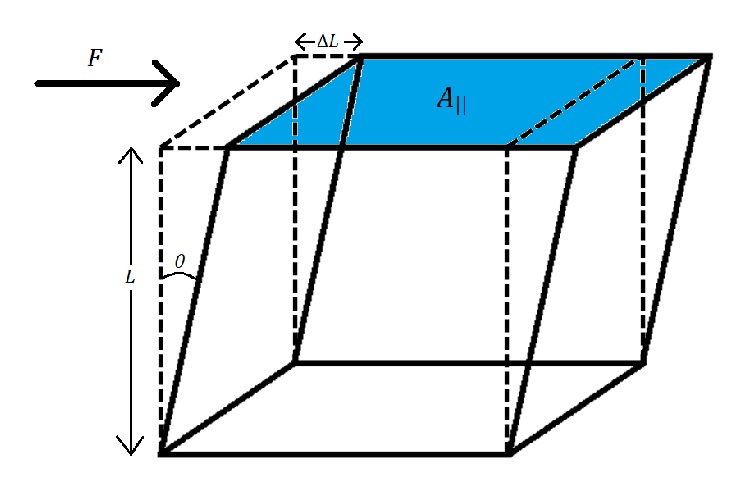
\includegraphics[width=\textwidth]{shear.eps}
                \caption{This is a picture of the shear modulus variables.}
            \end{minipage}
        \end{figure}
        \item When a longitudinal force stretches a wire, a lateral force also decreases its cross-sectional area. Poisson's ratio captures this effect and it's given by \[\sigma=\frac{\text{lateral strain}}{\text{longitudinal strain}}=\frac{-\Delta R/R}{\Delta L/L}=-\frac{L\Delta R}{R\Delta L}\]
        \item There are a few relations between these moduli. They are given below (memorize the ones in bold) \[\mathbf{Y=3B(1-2\sigma)}\]\[\mathbf{Y=2G(1+\sigma)}\]\[\sigma=\frac{3B-2G}{2G+6B}\]\[\frac9Y=\frac1B+\frac3G\]
        \item Change in length of a rod of length due to heating is $\Delta L=\alpha L\Delta T$ where $L$ is the initial length of the rod.
        \item Change in surface area of a body due to heating is $\Delta A=\beta A\Delta T\approx2\alpha A\Delta T$ where $A$ is the initial surface area of the body.
        \item Change in volume of a body due to heating is $\Delta V=\gamma V\Delta T\approx3\alpha V\Delta T$ where $V$ is the initial volume of the body.
        \item Internal stress induced in  rod due to heating is \[\frac F{A_\text{cross}}=Y\alpha\Delta T\]
        \item Volumetric energy density due to internal molecular elastic energy is given by \[u=\frac{\text{stress}\times\text{strain}}2=\frac Y2\times(\text{strain})^2=\frac{(\text{stress})^2}{2Y}\]
    \end{itemize}
    \section{Fluid Mechanics}
    \begin{itemize}
        \item Effect of pressure on the density of a real liquid: \[\rho=\frac mV\implies\rho\mathrm dV+V\mathrm d\rho=\mathrm dm\implies\frac{\Delta\rho}{\rho}=-\frac{\Delta V}V=\frac{\Delta P}B\] Note that in the above case $\mathrm dm=0$\[\rho'=\rho_0\left(1+\frac{\Delta P}B\right)=\rho_0(1+C\Delta P)\]
        \item Inside a fluid, pressure follows the relationship $P_2=P_1+\rho gh$. Also, things to remember: $\rho\text{Hg}=13.6\text{ g/mL}$, and $\tan\theta=\frac ag$
        \item For a container with a hole at depth $h$  below surface, speed of flow of water out of the hole is given by \[v=\sqrt{2gh}\] And the time taken to drop the water level height $H$  to $H'$  by water flowing out of a hole of area $A_0$ is \[t=\frac A{A_0}\sqrt{\frac 2g}\left(\sqrt H-\sqrt{H'}\right)\] Here $A$  is the area of the surface of the liquid.
        \item Surface energy of a liquid needed to create additional surface area (using a soap film or something) is $E=S\Delta A$ where $S$ is the surface tension. \textbf{Remember} that a soap film has 2 surface areas one on the back and one in the front, so calculate appropriately.
        \item Pressure inside a drop of liquid is given by \[P=P_0+\frac{2S}R\] Now, since this is a drop and not a bubble, there is only 1 area (the outer surface area). But a bubble has 2, an inner and an outer area, so for that, the equation simply becomes \[P=P_0+\frac{4S}R\] The case where it's an air bubble inside a liquid, is the same case as a drop. $P_0$  in above equations is outside pressure which may or may not be atmospheric pressure. For, spheres with outer and inner radii of $R$ and $r$ respectively, replace $2/R$  above with \[\frac 1R+\frac 1r\]
        \item \textbf{Height of rise of liquid due to capillary action}: imagine a liquid like water rises to a height $h$ with $R$ as meniscus' radius. The meniscus acts like an inverted air bubble inside a liquid with the internal pressure of the bubble being $P_\text{atm}$. Using the formula for air bubbles, the liquid's pressure just under the meniscus is \[P_\ell=P_\text{atm}+\frac{2S}R\] Pressure at bottom of this column (which is level with the liquid's surface outside of tube is given by $P_\text{atm}=P_\ell+\rho gh\implies P_\ell=P_\text{atm}-\rho gh$ Now, if the meniscus meets the walls at an angle $\theta$, then the radius of the tube is $R_\text{tube}=R\cos\theta$. Substituting all of this in, we get \[h=\frac{2S\cos\theta}{\rho gR_\text{tube}}\] Note that here we have assumed that atmospheric pressure does not change appreciably across the height $h$. Also, we have ignored the negative sign because we only want to deal with scalars. Note that for liquids like mercury in which cohesive forces are stringer than adhesive forces, $\theta>\pi/2\implies h<0$. Thus, these liquids dip instead of rising in a tube. Also, $hR$ is a constant, so if $h$  cannot increase (because tube is too short), then $R$ will increase to accommodate until meniscus goes flat. No overflow though, because capillary action cannot propel liquid in the air!
        \item Viscous force is given by \[F_v=-\eta A\frac{\mathrm dv}{\mathrm dh}\] where $A$ is the area at the level, $\eta$ is the fluid's viscosity, and $\mathrm dv/\mathrm dh$ is called the height velocity gradient.
        \begin{figure}[H]
            \centering
            \begin{minipage}[b]{0.4\textwidth}
                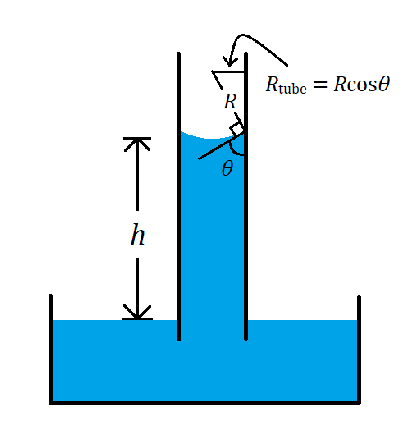
\includegraphics[width=\textwidth]{capillary.eps}
                \caption{How capillary action works.}
            \end{minipage}
            \hfill
            \begin{minipage}[b]{0.5\textwidth}
                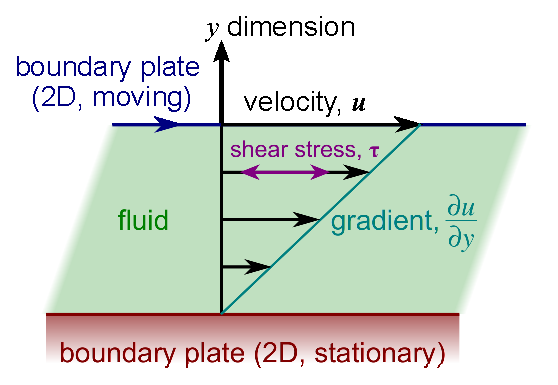
\includegraphics[width=\textwidth]{viscosity.eps}
                \caption{How viscosity works. Some variables might be different.}
            \end{minipage}
        \end{figure} Due to viscosity in a horizontal cylinder, fluid flow is highest in the center and slowest near the walls. So rate of fluid flow because of pressure difference $\Delta P$  across the cylinder's ends is \[\dot V=\frac{\pi r^4\Delta P}{8\eta L}\] where $L$ is the length of the pipe and $r$ is the radius. This is called Poiseuille's (PWA-ZUH-EE) Law; it can be rewritten as $\dot V=\Delta P/R_\ell$ where $R_\ell$ is liquid resistance. Series combination adds and parallel combination adds reciprocals.
        \item Drag force on a spherical object of radius $r$  moving at velocity $v$ through a viscous fluid is $F=6\pi\eta rv$. To find ``terminal" velocity of the spherical object, balance weight, buoyancy, and drag and is given by \[v_\text{term}=\frac{2r^2(\rho-\sigma)g}{9\eta}\] where $\sigma$ is the density of the medium and $\rho$ is the density of the object.
        \item Critical velocity above which flow turns from streamlined to turbulent is given by the formula \[v=\frac{\eta N_R}{2\rho R}\] where $N_R$ is called \textbf{\textit{Reynold's Number}} and $R$ is the pipe radius.
        \item In a pipe flowing with water, using conservation of mass, $m=\rho_\ell V=\rho_\ell vA_\text{cross}=\text{constant}$. Now, since liquids are incompressible, $\rho_\ell$ must remain constant, hence we get $\boxed{vA_\text{cross}=\text{constant}}$
        \item Bernoulli's Principle which is essentially a conservation of mass and energy is \[PV+mgh+\frac12mv^2=\text{constant}\]
    \end{itemize}
    \section{Thermodynamics}
    \begin{itemize}
        \item The heat of fusion of H$_2$O: 80 cal g$^{-1}$. Heat of vaporization of H$_2$O: 540 cal g$^{-1}$. 1 cal = 4.2 J.
        \item Equation of conduction through a rod of cross sectional area $A$ is \[\dot Q=kA\frac{\mathrm dT}{\mathrm dx}\] where $k$ is known as the material's coefficient of thermal conductivity.
        \item Conduction Law above can be rewritten as $\dot Q=\Delta T/R$ where $R$ is thermal resistance. Series combination adds and parallel combination adds reciprocals.
        \item Spectral absorptive power $\left(a_\lambda\right)$ is the ratio of the \textbf{power} absorbed to the power incident at wavelength $\lambda$.
        \item Spectral emissive power $\left(j^\star_\lambda\right)$  is the \textbf{power} per unit area emitted at a wavelength $\lambda$.
        \item \textbf{Kirchhoff's Law of Thermal Radiation}: for ALL objects, $\sfrac{j^\star_\lambda}{a_\lambda}$  is constant and equal to spectral emissive power of a perfect black body (PBB) at the same temperature and for the same wavelength.
        \item Emissive power $\left(j^\star\right)$ is the \textbf{total power} per area emitted at all wavelengths i.e. \[j^\star=\int_0^\infty j^\star_\lambda\text{ }\mathrm d\lambda\]
        \item Emissivity $\left(\epsilon\right)$ of a body is the ratio of its emissive power to the emmisive power of a PBB.
        \item Stefan-Boltzmann Law related emissive power of a PBB to it's temperature: \[j^\star=\sigma T^4\] where $\sigma=5.67\times10^8$ W m$^{-2}$K$^{-4}$ To apply this to all objects, you can simply multiply by the emissivity to get the full Stefan-Boltzmann Law: \[j^\star=\epsilon\sigma T^4\]
        \item Cooling by radiation is dictated by the following law: \[\dot T=\frac{A\sigma \epsilon}{mc}\left(T^4-T_S^4\right)\] where $A$ is the surface area, $T_S$ is the surrounding temperature, and $c$ is the specific heat capacity of the object.
        \item Newton's law of cooling gives the rate of cooling of an object through all methods but it is valid for only small temperature differences: $\boxed{\dot Q=bA\left(T-T_S\right)}$ Here $T_S$ is the surrounding temperature and $b$ is a constant.
        \item Wien's Displacement Law gives the wavelength that corresponds to the peak of a black body curve. For a given temperature, the wavelength of maximum intensity is $\boxed{2.88\times10^{-3}=T\lambda_\max}$
        \item The temperature change when an object is heated is given by $\Delta Q=mc\Delta T$ or by $\Delta Q=nc_m\Delta T$ where $c$ is the specific heat capacity and $c_m$ is the molar specific heat capacity. Also, $c_m=Mc$ where $M$ is the molar mass of the substance.
        \item The ideal gas law is $PV=KT$ where $K=Nk_B$. Here, $N$ is the number of particles of the gas and $k_B$ is the Botzmann constant. Clearly, $N=nN_A$ Substituting, we get $PV=nN_Ak_BT$ defining a new constant $R=N_Ak_B$, we get the familiar $PV=nRT$.
        \item Before proceeding further, we must define a few things: $c_{P,m}$ is the molar specific heat of a gas throughout some isobaric process and likewise, $c_{V,m}$ is the molar heat throughout some isochoric process. Something to \textbf{remember}: $\boxed{c_{P,m}-c_{V,m}=R}$ where $R$ is the universal gas constant. Do not forget that the above are \textit{molar} specific heats, that's a common mistake!
        \item If one has a mixture of $n_1,n_2,\dots,n_n$ moles of $n$ gases are, then \[c_{V,m}=\frac{\sum n_ic_{V,m,i}}{\sum n_i}\]\[c_{P,m}=\frac{\sum n_ic_{P,m,i}}{\sum n_i}\]
        \item Work done in expanding a gas is just force times distance which is just pressure times area times distance. However, area time distance is just volume. Thus, we get \[W=\int_{V_1}^{V_2}P\mathrm dV\]
    \end{itemize}\newpage
    \subsection{Laws of Thermodynamics}
    \begin{enumerate}[start=0]
        \item If body $A$ is in thermal equilibrium with body $C$, and so is body $B$, then bodies $A$ and $B$ are in thermal equilibrium with each other.
        \item Essentially a statement of conservation of energy $\boxed{\Delta U=\Delta Q-W}$ Here $\Delta U$ is the change in internal energy which depends on temperature. $\Delta Q$ is the energy/heat provided and $W$ is the work done by the gas. \textbf{Important}: $W>0$ if the work is done \textit{on} the system and $W<0$ is work is done \textit{by} the system.
        \item Total entropy of an isolated system cannot decrease with time and is constant if and only if all processes are perfectly reversible: $\Delta S\geq0$
        \item Essentially a statement of diffusion: \[\lim_{T\to0}S=\text{constant}\] where $T$ is the thermodynamic temperature of the system.
    \end{enumerate}
    \begin{itemize}
        \item To calculate $\Delta U$, you must measure the heat coming in the system while ensuring $W=0$. So to do this, you must use an isochoric process because that alone ensures $W=0$. And $\Delta Q=mc\Delta T$, but since this is an isochoric process, $\Delta Q=\boxed{\Delta U=mc_V\Delta T}$
    \end{itemize}
    \subsubsection{Isothermal Process}
    \quad \textbf{A process where the temperature of the system remains constant}
    \begin{itemize}
        \item $PV=nRT=\text{constant}\implies P_1V_1=P_2V_2$ which is also called Boyle's Law.
        \item To find slope of the PV graph, \[PV=k\implies P\mathrm dV+V\mathrm dP=0\implies\boxed{\frac{\mathrm dP}{\mathrm dV}=-\frac PV}\]
        \item Work done: \[W=\int_{V_1}^{V_2}P\mathrm dV=\int_{V_1}^{V_2}\frac{nRT}V\mathrm dV\implies \boxed{W=nRT\ln\left(\frac{V_2}{V_1}\right)=nRT\ln\left(\frac{P_1}{P_2}\right)}\]
        \item Since there is no change in temperature, $\Delta U=0$. Using 1$^\text{st}$ law of thermodynamics, \[\Delta Q=W=nRT\ln\left(\frac{V_2}{V_1}\right)\]
        \item To calculate the specific heat capacity of the gas: \[c=\frac{\Delta Q}{m\Delta T}\implies\boxed{c=\infty}\]
        \item To calculate the bulk modulus, \[B=-V\frac{\mathrm dP}{\mathrm dV}\implies\boxed{B=P}\]
    \end{itemize}\newpage
    \subsubsection{Adiabatic Process}
    \quad \textbf{A process where there is no exchange of heat}
    \begin{itemize}
        \item In an adiabatic process, $PV^\gamma=k$ where $k$ is a constant and $\gamma$ is called the adiabatic constant. The following equation (the derivation comes later) holds: $\gamma=c_{P,m}/c_{V,m}$.
        \item To find the slope of the graph, \[PV^\gamma=k\implies \gamma PV^{\gamma-1}\mathrm dV+V^\gamma\mathrm dP=0\implies\boxed{\frac{\mathrm dP}{\mathrm dV}=-\frac{\gamma P}V}\]
        \item Work done: \[W=\int_{V_1}^{V_2}P\mathrm dV=\int_{V_1}^{V_2}\frac k{V^\gamma}\mathrm dV\implies \boxed{W=\frac{k\left(V_2^{1-\gamma}-V_1^{1-\gamma}\right)}{1-\gamma}=\frac{R\left(T_2-T_1\right)}{1-\gamma}}\]
        \item Using 1$^\text{st}$ law \[\Delta U=-W=\frac{k_1\left(V_2^{1-\gamma}-V_1^{1-\gamma}\right)}{\gamma-1}=\frac{R\left(T_2-T_1\right)}{\gamma-1}\]
        \item To calculate the specific heat capacity of the gas, \[c=\frac{\Delta Q}{m\Delta T}\implies\boxed{c=0}\]
        \item To calculate the bulk modulus, \[B=-V\frac{\mathrm dP}{\mathrm dV}\implies\boxed{B=\gamma P}\]
    \end{itemize}
    \subsubsection{Isochoric Process}
    \quad \textbf{A process where the volume of the system remains constant}
    \begin{itemize}
        \item In an isochoric process \[\frac PT=\frac{nR}V\implies\frac{P_1}{T_1}=\frac{P_2}{T_2}\] This result is known as Gay-Lussac's Law.
        \item Since $\Delta V=0\implies W=0$. Using 1$^\text{st}$ law: \[\Delta Q=\Delta U=mc_V\Delta T\]
        \item To calculate the specific heat capacity of the gas, \[\Delta Q=mc_V\Delta T\implies c_V=\frac{\Delta Q}{m\Delta T}\implies\boxed{c=c_V>0}\] Here, to keep the volume constant, heating the gas must increase the temperature. Thus the signs of $\Delta Q$ and $\Delta T$ will always be the same.
        \item To calculate the bulk modulus, \[B=-V\frac{\mathrm dP}{\mathrm dV}\implies \boxed{B=-\infty}\]
    \end{itemize}
    \subsubsection{Isobaric Process}
    \quad \textbf{A process where the pressure of the system remains constant}
    \begin{itemize}
        \item In an isobaric process: \[\frac VT=\frac{nR}P\implies\frac{V_1}{T_1}=\frac{V_2}{T_2}\] This result is known as Charles' Law
        \item Since $P$ is constant, the integral for work simplifies to $W=P\Delta V=nR\Delta T$. As always, $\Delta U=mc_V\Delta T=nc_{V,m}\Delta T$, and using 1$^\text{st}$ law, $\Delta Q=\Delta U+W\implies\Delta Q=n\left(c_{V,m}+R\right)\Delta T\implies\Delta Q=mc_P\Delta T$.
        \item To calculate the specific heat capacity of the gas, \[\Delta Q=mc_P\Delta T\implies c_P=\frac{\Delta Q}{m\Delta T}\implies\boxed{c=c_P<0}\] Here, to keep the pressure constant, increasing temperature must result in heat being released. Thus the signs of $\Delta Q$ and $\Delta T$ will always be opposite.
        \item To calculate the bulk modulus, \[B=-V\frac{\mathrm dP}{\mathrm dV}\implies \boxed{B=0}\]
    \end{itemize}
    \subsubsection{Carnot Cycle}
    \begin{itemize}
        \item Thermal efficiency of any machine: \[\eta=\frac W{\Delta Q}\]
        \item In a closed-loop cycle, on a PV graph, the area inside the cycle is the total work done.
        \item An engine derives work from an exchange of heat from a hot reservoir to a cold reservoir. A refrigerator drives an exchange of heat from a cold reservoir to a hot reservoir, i.e. it \textit{requires external work}. A heat \textit{pump} derives an exchange of heat from a cold reservoir to a hot reservoir too, but the key difference is the environment. A heater keeps the system hot while surrounding is cold, so energy flows \textit{into} the system. A refrigerator keeps the system cool while the surrounding is hot, so energy flows \textit{out of} the system.
        \item \textbf{Important}: the Carnot Theorem states that no engine is more efficient than a Carnot engine between a hot and a cold reservoir of temperatures $T_1$ and $T_2$  respectively. The same hold for a Carnot heat pump and a Carnot refrigerator.
        \item For a Carnot engine, \[\eta_\text{Carnot}=1-\frac{T_L}{T_H}\]
        \item For a Carnot refrigerator, \[\eta_\text{Carnot}=\frac{T_L}{T_H-T_L}\]
        \item For a Carnot heat pump, \[\eta_\text{Carnot}=\frac{T_H}{T_H-T_L}\]
    \end{itemize}
    \subsection{Root Mean-Square Velocity (RMS)}
    \quad Imagine a particle moving in the positive $x$ direction with velocity $\vec{\mathbf v}=v_x\hat{\mathbf i}+v_y\hat{\mathbf j}+v_z\hat{\mathbf k}$. It will collide with the wall parallel to $yz$-plane which has an area $A$ (say). Its change in momentum will be $\Delta p=-2mv_x$ where $m$ is the mass of each particle. Now, in time $\Delta t$  a particle will collide with the wall if and only if it is within distance $v_x\Delta t$ of the wall. So, half the particles within a volume $Av_x\Delta t$ will collide (since half of them are equally likely to be moving away from the wall). If $\eta$  is the particle density (number of particles per unit volume), then $N=\frac 12\eta Av_x\Delta t$ particles will collide with the wall. Total change in momentum is \[\Delta p_\text{total}=N\Delta p=-m\eta A\left\langle v_x^2\right\rangle\Delta t\implies-\frac{\Delta p_\text{total}}{A\Delta t}=P=m\eta\left\langle v_x^2\right\rangle\] Note that in the above equation, we replaced $v_x^2$ with $\left\langle v_x^2\right\rangle$ which is just the mean square velocity of the particles (since not all will have the same $x$ component of velocity). Since gas is isotropic (meaning no direction is favored), the average of all 3 components should yield the same value, i.e. \[\left\langle v_x^2\right\rangle=\left\langle v_y^2\right\rangle=\left\langle v_z^2\right\rangle=\frac{\left\langle v_x^2\right\rangle+\left\langle v_y^2\right\rangle+\left\langle v_z^2\right\rangle}3=\frac13v_{\text{RMS}}^2\implies P=\frac13m\eta v_{\text{RMS}}^2\] Now, $m\eta=\rho$, thus, \[P=\frac 13\rho v_{\text{RMS}}^2\implies \boxed{v_\text{RMS}=\sqrt{\frac{3P}\rho}}\] Using the ideal gas law, a lot of given values can help you find $v_\text{RMS}$.
    \begin{itemize}
        \item Total kinetic energy of each particle is: \[\boxed{KE=\frac12mv_\text{RMS}^2}=\frac{3mP}{2\rho}=\frac{3mnRT}{2M}=\frac{3nN_Ak_BT}{2N}\implies\boxed{KE=\frac32k_BT}\]
        \item Total kinetic energy of the gas is simply by multiplying the above equation by $N$: \[KE_\text{total}=\frac12Mv_{\text{RMS}}^2=\frac32Nk_BT\]
        \item The rate of diffusion of a gas $r$ is given by \[r\propto\frac1{\sqrt\rho}\implies\frac{r_1}{r_2}=\sqrt{\frac{\rho_2}{\rho_1}}\]
        \item Other than $v_\text{RMS}$, there is also the most probable velocity $\left(v_\text{mp}\right)$ and average velocity of the particles $\left(\langle v\rangle)$. They are given by Maxwell's speed distribution which is too advanced, by their values are \[v_\text{mp}=\sqrt{\frac{2P}\rho}=\sqrt{\frac23}v_\text{RMS}\approx0.8v_\text{RMS}\]\[\langle v\rangle=\sqrt{\frac{8P}{\pi\rho}}=\sqrt{\frac8{3\pi}}v_\text{RMS}\approx0.9v_\text{RMS}\]
    \end{itemize}
    \subsubsection{Law of Equipartition of Energy}
    Each degree of freedom (DOF) contributes the same amount of \textit{internal} energy to each particle. This energy is $\frac12k_BT$. Now, you might recognize this as the same as the one we calculated above, and that is because our derivation was for the simplest case, with only 1 DOF.
    \begin{itemize}
        \item \textbf{Important}: the number of DOFs that a gas has is given by $D=3N-B$ where $N$ is the number of atoms per particle. So for a monoatomic gas, $N=1$. $B$ is the number of bonds present, so for a diatomic gas, $B=1$.
        \item Now, let $n$  moles of a gas have $f$ DOFs. Then, \[U=\frac12k_BT\times nN_A\times f=\frac f2nRT\] To make a small change in internal energy $\mathrm dU$  at constant volume, corresponding rise in temperature is \[\mathrm dT=\frac{\mathrm dU}{nc_{V,m}}\implies nc_{V,m}=\frac{\mathrm d}{\mathrm dT}\left(\frac f2nRT\right)\implies\boxed{c_{V,m}=\frac{fR}2}\] Now, $c_{P,m}=c_{V,m}+R$, thus we get, \[\boxed{c_{P,m}=R\left(1+\frac f2\right)}\] Now, we have already seen that the adiabatic constant is just $c_{P,m}/c_{V,m}$, so, \[\boxed{\gamma=\frac{c_{P,m}}{c_{V,m}}=1+\frac2f}\]
        \item If $n_1,n_2,\dots,n_n$ moles of $n$ gases with DOFs $f_1,f_2,\dots,f_n$ and temperatures $T_1,T_2,\dots,T_n$ respectively are mixed, then \[f_\text{equiv}=\frac{\sum\left(f_in_i\right)}{\sum n_i}\]\[T_\text{final}=\frac{\sum\left(f_in_iT_i\right)}{\sum \left(f_in_i\right)}\]
        \item Mean free path in a gas is $\ell_\text{mfp}=\left(\sqrt2\eta\sigma\right)^{-1}$. Here, $\eta$ is the particle density again, and $\sigma$ is the \textit{effective} cross-sectional area of a particle. Two particles will only collide if their cross sectional areas intersect, i.e. if another particle strays within an area of $\pi(2r)^2=\pi d^2$ of another particle.
        \item Pressure, temperature, internal energy, and entropy are state functions.
        \item To calculate entropy, the equation is \[\Delta S=\int_{Q_1}^{Q_2}\frac{\mathrm dQ}T\]
    \end{itemize}\newpage
    \subsubsection{Statistical Analysis of Entropy}
    \quad If there are $N$ identical particles in a box, then there are $N+1$ different configurations where there are $n_1$ particles in the left half and $n_2$ particles in the right half of the box, i.e. $(n_1,n_2)\in\{(N,0),(N-1,1),\dots,(0,N)\}$. There are \[W=\frac{N!}{n_1!n_2!}\] ways (called microstates) to arrange the particles for each configuration. Now, the entropy of the $i^\text{th}$ configuration is given by $S_i=k_B\ln W_i$. Each of these $W$ microstates are equally likely, but since some configurations have more microstates not all configurations are equally likely. So the first configuration $(N,0)$ where all the particles are in the left half has only 1 microstate. So for this configuration, this particular microstate is guarenteed (since that's the only \textit{possible} microstate). \textit{But} the configuration itself has a very low probability since it is nearly impossible for all the particles to randomly end up in the left half of the box. Thus, to find the entropy at any point in time, take the configuration that the particles are in, and apply the above formula. So, in our unlikely example, the entropy is 0. This is why entropy of a system decreasing is so unlikely because configurations with low entropy are just \textit{naturally} so unlikely. Meanwhile the configuration $(N/2,N/2)$ where all particles are split evenly in half, has many more microstates and is most likely with maximum entropy.
    \section{Waves}
    \begin{itemize}
        \item The equation of a wave is \[y\left(x,t\right)=A\sin\left[\omega\left(t-\frac xv\right)\right]=A\sin\left(\omega t-kx\right)=A\sin\left(\frac{2\pi}Tt-\frac{2\pi}\lambda x\right)  \] There are a few things to discuss here. Firstly, this equation describes a string wave where $y$ is the height of the wave above the median, $t$ is the time, and $x$ is the distance \textit{along} the wave. Here $k$ is called the wave number, $v$ is the velocity of the wave. Now, something to remember:\[k=\frac\omega v=\frac{2\pi}\lambda\]
        \item Velocity of a particle (in the $y$-direction): \[v_p=\frac{\mathrm d}{\mathrm dt}\left[A\sin\left(\omega t-kx\right)\right]=A\omega\cos\left(\omega t-kx\right)\]
        \item Slope of wave at any point: \[\frac{\mathrm dy}{\mathrm dx}=m=-Ak\cos\left(\omega t-kx\right)\]\[\frac{v_p}m=-\frac\omega k=-v\implies v_p=-mv\]
        \item Using the same consideration as above, you get $\boxed{\ddot y=v^2y''}$ Just like with S.H.M., if this condition is satisfied, then the equation of $y(x,t)$  is a wave equation. Another thing to remember is \[\phi=\frac{2\pi}\lambda\Delta x\]
        \item The tension on a string has an effect on the velocity of the wave, i.e. $T=\mu v^2$ where $\mu$ is the linear mass density and $T$ is the string's tension.
        \item For a vertically hanging, massive string, acceleration of wave velocity up the string is constant: $v=\frac g2$.
        \item The power transferred through the wave \[P(x,t)=TA^2k\omega\cos^2\left(\omega t-kx\right)\] where $P$ is the power through point $x$. To find the average power, find the average of the $\cos^2$ function (which is $\sfrac12$), thus we get, \[\langle P\rangle=\frac12\omega kTA^2\].
        \item For any string, $m=sL\rho$ where $s$ is the cross-sectional area, of the string and $\rho$ is the string's density. Clearly, $\mu=m/L=s\rho$; substituting this into the above equation, \[\langle P\rangle=\frac12\omega k\left(s\rho v^2\right)A^2\implies I=\frac{\langle P\rangle}s=\frac12\rho v\omega^2A^2\] where $I$ is the intensity of the wave.
        \item The elastic potential energy is maximum at the median and minimum at the crest/trough since string is stretched at the median. Likewise the kinetic energy is also maximum at median.
        \item Two points $A$ and $B$ are apart by a distance $\mathrm dx$ and their corresponding points on the wave $A'$ and $B'$ are apart by a vertical distance $\mathrm dy$. Elongation in the string is $\mathrm dl=\sqrt{\mathrm dx^2+\mathrm dy^2}-\mathrm dx\implies\mathrm dl=\mathrm dx\left(\sqrt{1+\left(y'\right)^2}-1\right)$ Multiplying by force $T$ and using binomial approximation we get \[T\mathrm dl=\mathrm dU=\frac{T\mathrm dx}2\left(y'\right)^2\implies U'=\frac12T(y')^2\]
        \item When a wave goes from a denser medium into a rarer medium, there is no bounce, however when it goes into a denser medium, part of the wave continues and another wave is reflected backwards. When a pulse reflects off a denser medium there's a phase change of $\phi=\pm\pi$, i.e. pulse flips upside-down. Since energy must be conserved, the following equation holds: $A_i+A_r=A_t$ where $A_i$ is the incident wave, $A_r$ is the reflected wave, and $A_t$ is the transferred wave's amplitude, respectively.
    \end{itemize}
    ETOOS Waves, Lesson 8
    \begin{itemize}
        \item The energy is divided as, \[A_t=\frac{2v_2}{v_1+v_2}A_i\]\[A_r=\frac{v_2-v_1}{v_1+v_2}A_i\] where $v_1$ is the wave velocity in first (rarer) medium, and $v_2$ is the velocity in the second medium.
        \item Standing waves are the interference of two identical waves going in opposite directions. Standing waves are basically like ripples: they oscillate in place. The equation of a standing wave is $y=y_1+y_2$ where $y_1$ and $y_2$ are the equations of the original waves, i.e. \[y=A\sin\left(\omega t-kx\right)+A\sin\left(\omega t+kx\right)=2A\sin\left(\omega t\right)\cos\left(kx\right)\]
        \item For some point $x$, the equation becomes $y(t)=C\sin\left(\omega t\right)$ which is the S.H.M. equation. Thus, in a standing wave, each point performs harmonic motion. Note that if there is a phase difference between the waves (which there usually is) then, it'll be some multiple of $\frac{\pi}2$ to make the math easier. In reality, it can be anything but for competitions, it's an easier value. Then the equation of the standing wave can made with \textit{any} combination of sine  and cosine. So, $2A\cos\left(\omega t\right)\cos\left(kx\right)$ is another correct general equation for standing waves. Also note that in the above equation, $2A$ can be replaced with $A_0$ where $A_0$ is the maximum amplitude of the standing wave. Thus, the standing wave equation becomes \[\boxed{y=A_0\sin(\omega t)\cos(kx)}\] Thus, there are some points that always stay in place on the median. These are known as the \textit{nodes}. Conversely, those points that have maximum amplitude are known as \textit{antinodes}.
        \item The energy within each loop (which is the region between two adjacent nodes) of a standing wave is constant. When the loop is fully stretched, i.e. the antinode is at its greatest amplitude, all the energy of the loop is potential. Conversely, when loop lies along the median, all the energy is kinetic. At such a moment, take a small element a distance $x$ from the left node and thickness $\mathrm dx$. Then, the mass of this element is $\mathrm dm=\mu\mathrm dx$. Kinetic energy is \[\mathrm dK=\frac12\left(\mathrm dm\right)v^2=\frac12\mu v^2\mathrm dx\] In S.H.M., $v=\omega\sqrt{A^2-x^2}$. Since distance from mean position is 0, $v^2=\omega^2A^2$. Note that this $A$  isn't the same $A$ as the one that appears in the standing wave equation. The above $A$ is specific to the element. Here, $A$ is equal to $A_0\sin(kx)$ assuming the equation is $y=A_0\sin(kx)\cos(\omega t)$. Thus we get the differential equation \[\mathrm dK=\frac12\mu\omega^2A_0^2\sin^2(kx)\mathrm dx\] Substituting,$k=2\pi/\lambda$, we get, \[\mathrm dK=\frac12\mu\omega^2A_0^2\sin^2\left(\frac{2\pi x}{\lambda}\right)\mathrm dx\] To solve, remember that two adjacent nodes are separated by half a wavelength. Solving, we get, \[\int_0^K\mathrm dK=\frac12\mu\omega^2 A_0^2\int_0^\frac\lambda2\sin^2\left(\frac{2\pi x}{\lambda}\right)\mathrm dx\implies\boxed{K=\frac18\mu\lambda\omega^2A_0^2}\] That is the energy in each loop and since all the loops contain equal energy, multiplying it by the number of loops, we can get the energy in the whole standing wave.
        \item In a string standing wave that is bound on both ends, there can be only an integer number of loops. If there's 1 loop, it's called the \textbf{\textit{fundamental mode}} of the standing wave. In this case, $\lambda=2L$ where $L$ is the length of the string. The frequency in this case is called the \textbf{\textit{fundamental frequency}}. It's given by, \[\nu_{0,\text{bound}}=\frac v{2L}=\sqrt{\frac T{3mL}}\] After the fundamental mode, there come 2 nodes. This is called the 2$^\text{nd}$ harmonic or the 1$^\text{st}$ overtone. It has a frequency \[\nu_{1,\text{bound}}=2\nu_{0,\text{bound}}=\frac vL\] And in general, the $n^\text{th}$ harmonic or the $(n-1)^\text{th}$ overtone has $n$ nodes and has a frequency \[\boxed{\nu_{n-1,\text{bound}}=n\nu_{0,\text{bound}}=\frac{nv}{2L}}\]
        \item In the case where there's one end free on the string, the free end will become the antinode. Here, the first case will be when \[\lambda=4L\implies\nu_{0,\text{free}}=\frac v{4L}\]. These are the fundamental mode and fundamental frequency for one-end-free case. The next case has three-quarters of a wavelength, so, \[\nu_{1,\text{free}}=\frac{3v}{4L}\] This means that these frequencies are odd multiples of $\nu_{0,\text{free}}$ and even multiples of $\nu_{0,\text{bound}}$. For when there is one end free, there are no 2$^\text{nd}$ or 4$^\text{th}$ harmonics, since those multiples are not possible. Thus, for the case where 1 end is free has ``missing" harmonics.
        \item If an object performs oscillatory motion at frequency $\nu_0$, and a force is applied at regular intervals at frequency $\nu_\text{res}$, then it is defined as \textit{resonance} if and only if $\nu_0=n\nu_\text{res}$ where $n$ is an integer.
    \end{itemize}
    \subsection{Sound Waves}
    \begin{itemize}
        \item In sound waves, compression is where pressure is higher ($P_0+\Delta P$) and rarefaction is where pressure is lower ($P_0-\Delta P$). Thus, if you graph pressure-vs-$x$, you get a sinusoidal wave. The graph of the particles' displacement-vs-$x$ is also a sinusoidal wave that lags behind by a phase of $\frac\pi2$ behind the pressure wave. So, the region of maximum rarefaction and compression is where the particles' displacement from their mean positions is 0. At the points where pressure is $P_0$ is where displacement is maximum.
    \end{itemize}
    Resnick and Halliday Part 1 \textbf{Pg. 499-502}
    \begin{itemize}
        \item Speed of sound wave in a gas of bulk modulus $B$ and density $\rho_0$is given by \[v=\sqrt{\frac B{\rho_0}}\] In a solid, $B$ is replaced with $Y$, the Young's modulus. When sound goes through a gas, it causes adiabatic expansion. From thermodynamics, we know for a gas undergoing adiabatic expansion $B=\gamma P$, so \[\boxed{v=\sqrt{\frac B{\rho_0}}=\sqrt{\frac{\gamma P}{\rho_0}}}\] You can also adopt an isothermal expansion as an approximation. For an isothermal approximation, the sound velocity deviates from the adiabatic case and is, \[\sqrt{\frac{P_0}{\rho_0}}\] because for isothermal processes, $\gamma=1\implies B=P$.
        \item If equation of a sound wave is $x_p=A\sin\left(\omega t-kx\right)$ where $x_p$ is the particles' displacement then pressure equation will be $\boxed{P=P_0\cos\left(\omega t-kx\right)}$ \textbf{Important}: $\boxed{P_0=kBA}$ The sine function switched to a cosine and vice-versa too.
        \item Going by the string wave's logic, in a standing sound wave (in a pipe), a pressure \textit{node} is a particle-displacement \textit{antinode}. In a pipe, the closed end is a displacement \textit{node}, or a pressure \textit{antinode}. Otherwise, all concepts of standing waves apply. Pipes open (or closed) at both ends have frequencies \[\nu_n=\frac{(n+1)v}{2L}\] where $L$ is the length of the pipe. A pipe open at one end and closed at the other has frequencies \[\nu_n=\frac{(2n+1)v}{4L}\]
        \item Intensity of sound waves is given by \[I=\frac{P_0^2}{2\rho v}\] Now, since sound waves are not as well-defined as strings, when they exit the pipe, the node is not \textit{exactly} at the pipe's end. Thus, there is need of length correction. Experimentally, it has been found to be \[\boxed{L_\text{eff}=L+\frac35R}\] where $R$ is the pipe's radius.
        \item \textbf{Not very important}: if 2 waves have equations $P_1=P_{0,1}\sin\left(\omega t-kx\right)$ and $P_2=P_{0,2}\sin\left(\omega t-kx+\phi\right)$ at a point, there will be interference at that point and the resultant equation would be $\vec{\mathbf P}=\vec{\mathbf P_1}+\vec{\mathbf P_2}$ which equals \[P=P_{0,R}\left(\omega t-kx+\delta\right)\] The resultant wave as a phase difference and a new amplitude given by, \[P_{0,R}^2=P_{0,1}^2+P_{0,2}^2+2P_{0,1}P_{0,2}\cos\phi\]\[\tan\delta=\frac{P_{0,2}\sin\phi}{P_{0,1}+P_{0,2}\cos\phi}\]
        \item The intensity is $I\propto A^2$, i.e. $I=kP_0^2$ Plugging in the corresponding values of $P$ into the equations above we get, and this is \textbf{important}: \[\boxed{I_R=I_1+I_2+2\sqrt{I_1I_2}\cos\phi}\]
        \item Loudness, measured in Bel is given by \[\Delta B=\log_{10}\left(\frac I{I_0}\right)\] Note that loudness is relative, so this equation really tells how the difference in loudness between a sound (of intensity $I$) and a reference sound (of intensity $I_0$). For most cases, the value of $I_0$ is set to 10$^{-12}$. To measure in dB, simply multiply the value of B by 10.
        \item Beats are an interference pattern of 2 waves of similar frequencies which is \textit{perceived} as a sound that periodically changes its volume. The frequency of this change in volume is $\boxed{\nu_B=\nu-\nu_1}$ where $\nu_1$ and $\nu_2$ are the frequencies of the original waves.
        \item Doppler effect: \[\boxed{f_\text{dopler}=\left(\frac{v_\text{wave}\pm v_\text{obs,r}}{v_\text{wave}\pm v_\text{source,r}}\right)f_0}\] where all velocities are radial along the line of travel of the wave. Both source and observer velocities are taken positive in the direction \textit{opposite} to the wave. So if the wave is going to the right, the \textit{left} will be taken as positive for all values.
    \end{itemize}
    \section{Electromagnetism}
    \subsection{Electrostatics}
    \begin{itemize}
        \item Coulomb's law: \[\vec{\mathbf F}=\frac1{4\pi\varepsilon}\frac{q_1q_2}{r^2}\hat{\mathbf r}\] In the above equation $\varepsilon$ is the absolute permittivity of medium and is given by $\varepsilon=\varepsilon_0\kappa$. Now, $\varepsilon_0$ is the permittivity of free space or vaccum and $\kappa$ is the relative permittivity (also called the dielectric constant). Note that $\varepsilon_0\approx9\times 10^{-12}$ F m$^{-1}$.
        \item The electric field at a point is simply a measure of the force felt by a unit test charge at that point.
        \item The electric field due to a rod of charge $q$ and length $L$ at a point at distance $x$ from the end of the rod is \[\vec{\mathbf E}=\frac{kq}{x\left(x+L\right)}\] Note that the point must lie on the line that goes through the rod along its length.
    \end{itemize}
    \begin{figure}[H]
        \centering
        \begin{minipage}[b]{0.5\textwidth}
            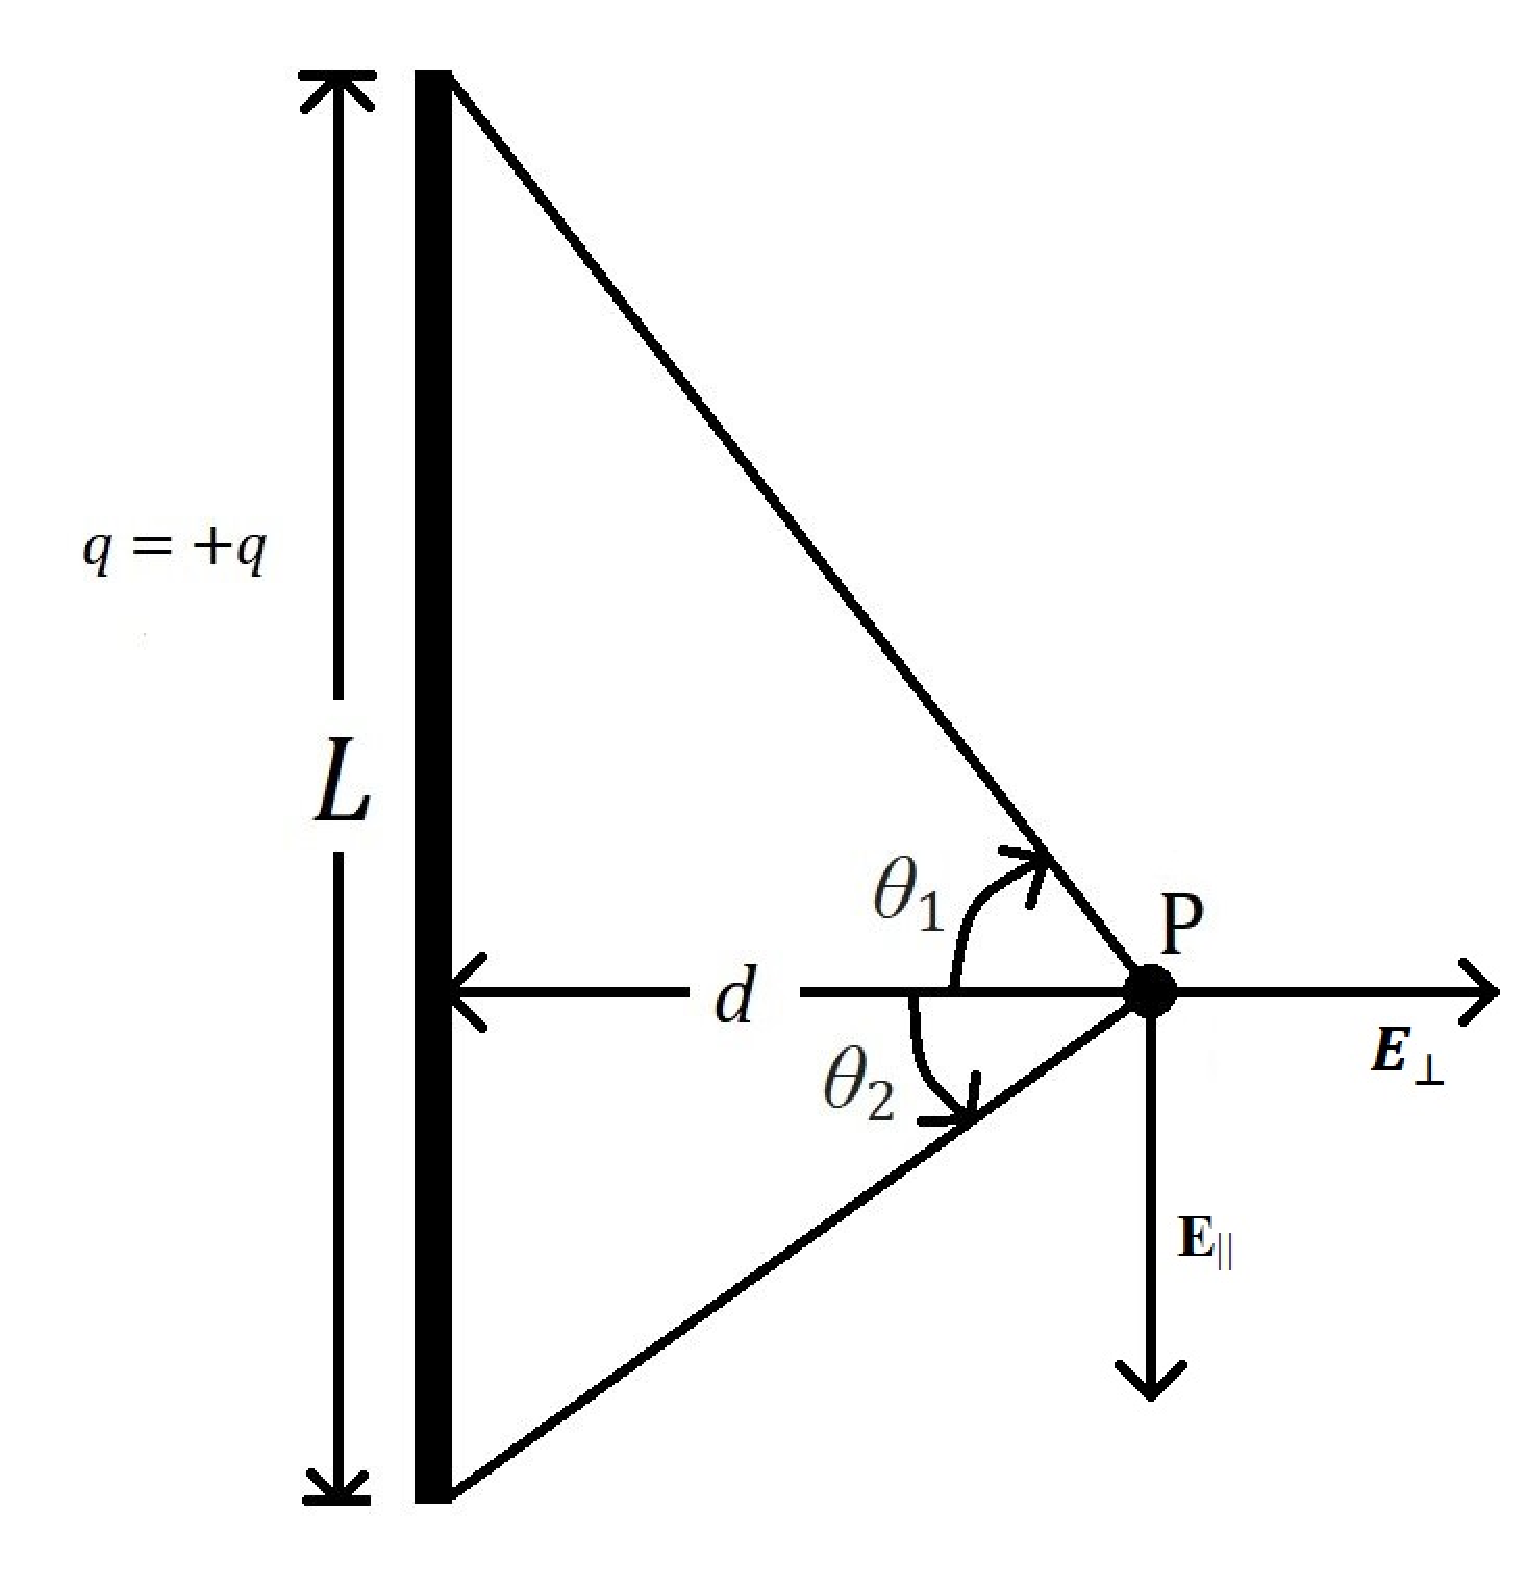
\includegraphics[width=\textwidth]{rod.eps}
            \caption{This is a picture of the rod's variables.}
        \end{minipage}
    \end{figure}
    \begin{itemize}
        \item The component of the electric field parallel to the rod at point $P$ in the case above is \[\boxed{\vec{\mathbf E}_{\parallel}=\frac{kq}{dL}\left(\cos\theta_2-\cos\theta_1\right)}\] And the component of electric field intensity perpendicular to the rod is \[\boxed{\vec{\mathbf E}_{\perp}=\frac{kq}{dL}\left(\sin\theta_1+\sin\theta_2\right)}\] \textbf{Note}: here $\theta_2$  is \textit{counterclockwise} from $\vec d$, i.e. below the line, so keep appropriate signs! Also if $\theta_2>\theta_1$, then $\vec{\mathbf E}_{\parallel}$ will point upwards.
        \item Electric field due to a circular arc of angle $\phi$, radius $R$, and charge $q$ is \[\boxed{\vec{\mathbf E}=\frac{2kq}{\phi R^2}\sin\frac{\phi}2}\]
        \item The electric field at a point on the axis of a ring of radius $R$, charge $q$ at a distance $x$ from the center is \[\boxed{\vec{\mathbf E}=\frac{kqx}{\left(x^2+R^2\right)^\frac32}}\] Maximum of $\|\vec{\mathbf E}\|$ occurs at $x=\pm R/{\sqrt2}$.
        \item Field due to a disk (calculated by integrating over rings from $r=0$ to $r=R$) along its axis is \[\vec{\mathbf E}=\frac{\sigma}{2\varepsilon}\left(1-\frac x{\sqrt{x^2+R^2}}\right)\] Under the special case $R\gg x$ (same as an infinite plane) \[\boxed{\vec{\mathbf E}_\text{plane}=\frac\sigma{2\varepsilon}}\] Same results under the special case $x\ll R$ (same as being near the disk). Note that although these cases may be mathematically identical, they are physically different.
        \item \textbf{NOTE:} inside a \textit{conductive} body the charge is \textit{always} on the surface and inside the body, $\boxed{\vec{\mathbf E}_\text{net}=0}$.
        \item Electric flux is the measure of the electric field through a surface, i.e. \[\boxed{\Phi_E=\vec{\mathbf E}\cdot\vec{\mathbf A}}\] Here $\vec{\mathbf A}$ is the area vector and The OUTER SURFACE is taken as positive for $\vec{\mathbf A}$. $\Phi_E$ is a scalar measured in Nm$^2$ C$^{-1}$ and is better defined with calculus: \[\boxed{\Phi_E=\iint_S\vec{\mathbf E}\cdot\mathrm d\vec{\mathbf A}}\]
        \item \textbf{Gauss' Law}: total flux through \textit{any} \textbf{\textit{closed}} surface (\textit{Gaussian} surface) that \textit{encloses} a \textbf{net} charge $q$ is $\Phi_E=q/\varepsilon$. Note that charge on the surface does \textbf{not} count. Gauss' Law is \textbf{\textit{Maxwell's First Equation}} and written more formally as \[\boxed{\oiint_{\partial\Omega}\vec{\mathbf E}\cdot\mathrm d\vec{\mathbf A}=\frac1\varepsilon\iiint_\Omega\rho\text{ }\mathrm dV}\implies\boxed{\vec{\mathbf{\nabla}}\cdot\vec{\mathbf E}=\frac\rho\varepsilon}\] Here the subscripts on the integrals simply represent that the volume to be integrated on the right-hand side is enclosed by the surface to be integrated on the left-hand side; the del represents the divergence of the electric field, and it returns a scalar. The divergence operator is defined as, \[\boxed{\vec{\mathbf{\nabla}}\cdot\vec{\mathbf{F}}=\frac{\partial F_x}{\partial x}+\frac{\partial F_y}{\partial y}+\frac{\partial F_z}{\partial z}}\]
        \item For a cone, that has a charge $q$ placed at its apex, all of the electric field lines exit through the base since all others do not every enter the cone. Thus, for a cone \[\boxed{\Phi_{E,\text{cone}}=\frac q{2\varepsilon}\left(1-\cos\theta\right)}\] Here, $\theta$ is the semi-vertical angle of the cone.
        \item Just like with gravity, Newton's Shell Theorem also applies to electrostatic. Note that earlier it was states that a conductive body holds all of its charge at its surface, i.e. a hollow body and a conducting body are identical in terms of the placement of charge.
        \item Electric field of an \textbf{\textit{insulating}} sphere of radius $R$ and charge $q$ at distance $r$ ($r<R$) from the center is \[\boxed{\vec{\mathbf E}=\frac{kqr}{R^3}}\]
        \item If a spherical cavity exists inside a sphere of charge $q$ and radius $R$ and the vector from the sphere's center to the cavity's center is $\vec{\mathbf a}$, then electric field at any point inside the cavity is \[\boxed{\vec{\mathbf E}=\frac{kq}{R^3}\vec{\mathbf a}}\]
        \item Electric potential at a point due to a charge $q$ is just the potential energy per unit test charge, i.e. \[V=\frac{kq}r\]
        \item \textbf{\textit{Electric potential decreases if you follow the electric field in its direction.}} In other words, electric potential is given by \[\boxed{\Delta V=V_B-V_A=-\int_A^B\vec{\mathbf E}\cdot\mathrm d\vec{\mathbf r}}\] This means that all along a curve that is perpendicular to the net electric field at all points, the voltage remains constant.
        \item Self energy is the energy contained in a charged body on account of the arrangement of its elementary charges. To calculate self energy of a conducting sphere of charge $Q$, and radius $R$, imagine the sphere already has charge $q$ and you want to add charge $\mathrm dq$. Then, work required is \[\mathrm dW=\Delta V\mathrm dq=\frac{kq}R\mathrm dq\implies\int_0^W\mathrm dW=\frac kR\int_0^Qq\mathrm dq\implies W=\boxed{E_\text{self}=\frac{kQ^2}{2R}}\]
        \item Energy density due to an electric field is given by \[\boxed{\rho_E=\frac12\varepsilon{\mathbf E}^2}\] To calculate self energy of a solid \textbf{\textit{insulating}} sphere, we need to calculate the energy \textit{inside} the sphere since the energy on the outside will be the same as a conducting sphere $\left(\frac{kq^2}{2R}\right)$. Take an elementary shell of radius $r$ $(r<R)$ and thickness $\mathrm dr$. Energy in the shell is $\mathrm dE_\text{in}=\rho_E\mathrm dV$. Now, $\mathrm dV=4\pi r^2\mathrm dr$ and \newline$\rho_E=\frac12\varepsilon{\mathbf E}^2$, i.e. $\mathrm dE_\text{in}=2\pi\varepsilon{\mathbf E}^2r^2\mathrm dr$. Now, $\vec{\mathbf E}$ remains constant inside the elementary shell and for an insulating sphere, at distance $r$ from the center, \[\mathbf E=\frac{qr}{4\pi\varepsilon R^3}\] Plugging all of this in, we get, \[\mathrm dE_\text{in}=\frac{q^2r^4\mathrm dr}{8\pi\varepsilon R^6}\implies E_\text{in}=\frac{q^2}{8\pi\varepsilon R^6}\int_0^Rr^4\mathrm dr=\frac{kq^2}{10R}\] Adding the inner and outer energies, \[E_\text{in}+E_\text{out}=\frac{kq^2}{10R}+\frac{kq^2}{2R}\implies\boxed{E_\text{self}=\frac{3kq^2}{5R}}\]
        \item Charge density is inversely proportional to radius of curvature. So in the \textit{\textbf{absence}} of an \textit{external electric field}, sharp points have high $\sigma$ and high $\vec{\mathbf E}$. When connecting 2 spheres, (spheres 1 and 2) their \textit{electric \textbf{potentials}} are equalized because charge always tries to go towards lower potential. You can think of it as them wanting to follow the electric field lines, or as nature's tendency towards lowest potential energy. So, doing a little math, \[\boxed{\frac{q_1}{q_2}=\frac{R_1}{R_2}\implies\frac{\sigma_1}{\sigma_2}=\frac{R_2}{R_1}}\]
    \end{itemize}
    \subsubsection{Electric dipole}
    An electric dipole is a pair of equal and opposite point charges $q$ and $-q$, separated by a distance (typically taken to be $2a$).
    \begin{itemize}
        \item Electric dipole moment is defined to be $\boxed{\vec{\mathbf p}=2q\vec{\mathbf a}}$ where $\vec{\mathbf a}$ points \textit{from} the negative charge \textit{to} the positive charge.
    \end{itemize}
    \begin{figure}[H]
        \centering
        \begin{minipage}[b]{.4\textwidth}
            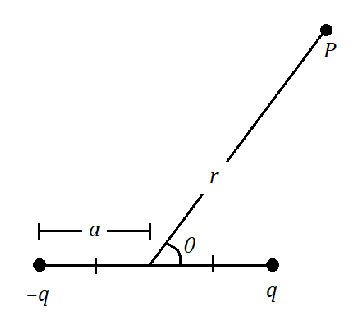
\includegraphics[width=\textwidth]{dipole.eps}
            \caption{This is a dipole.}
        \end{minipage}
    \end{figure}
    \begin{itemize}
        \item Electric potential at a point $P$ due to the dipole given that $p=\|\vec{\mathbf p}\|$ and $r\gg2a$ is \[\boxed{V_P=\frac{kp\cos\theta}{r^2}}\] Note that this is basically a scalar field given in polar co-ordinates (by the way, polar co-ordinates are just the 2D analogue of spherical co-ordinates). We know $\vec{\mathbf E}=-\vec\nabla V$ since all of their relation are analogous to potential energy and force. Now, \[\vec{\mathbf E}_P=-\frac{\partial V}{\partial r}\hat{\mathbf r}-\frac{\partial}{\partial\theta}\left(\frac Vr\right)\hat{\mathbf{\theta}}=\boxed{-\frac{2kp\cos\theta}{r^3}\hat{\mathbf r}+\frac{kp\sin\theta}{r^3}\hat{\mathbf{\theta}}}\] Now because of complex math reasons, these are also the magnitudes of the components of $\vec{\mathbf E}$ along $\vec r$ and perpendicular to $\vec r$, respectively. So, \[\boxed{\vec{\mathbf E}_r=-\frac{2kp\cos\theta}{r^3}}\]\[\boxed{\vec{\mathbf E}_\theta=\frac{kp\sin\theta}{r^3}}\]\[\boxed{\|\vec{\mathbf E}_P\|=\frac{kp}{r^3}\sqrt{1+3\cos^2\theta}}\] The direction of this electric field is just \[\boxed{\tan\alpha=\frac{\|\vec{\mathbf E}_\theta\|}{\|\vec{\mathbf E}_r\|}=\frac12\tan\theta}\]
        \item If placed in a uniform electric field, net force on a dipole is 0 since both charges are equally attracted and repelled. However, the torque may or may not be present because torque is $\boxed{\vec{\mathbf{\tau}}_E=\vec{\mathbf p}\times\vec{\mathbf E}}$
        \item Potential energy of a dipole in an external electric field is $\boxed{U_{E,\text{dipole}}=-\vec{\mathbf p}\cdot\vec{\mathbf E}}$
    \end{itemize}
    ETOOS Electrostatics (Pressure)
    \begin{itemize}
        \item When charge is placed on a conducting/hollow sphere, it repels each other and the surface of the sphere comes under tension. This electrostatic pressure is given by \[\boxed{P_E=\frac{\sigma^2}{2\varepsilon}}\]
    \end{itemize}
    \subsubsection{Conductor With a Cavity}
    \begin{itemize}
        \item Imagine you have a cavity of arbitrary shape in a conductor of arbitrary shape. If you place a charge $q_0$ inside the cavity, the inner surface (cavity's surface) will become negatively charged and outer surface will distribute positive charged. But if you move $q_0$ within the cavity, the negative charge will also move to compensate but the outer positive charge will not move. It will become independent of the inner negative charge. Conversely, any external electric field will move the outer surface charge to compensate and the negative charge on cavity surface and $q_0$ will remain unaffected. This is electric shielding.
        \item If you bring 2 conducting plates (one with charge $q$ and another with 0 charge), the charged plates divides its charge among its 2 surfaces into $q/2$ and the uncharged plate is polarized by induction. The surface facing the charged plate gets a charge of $-q/2$ and the outward-facing surface gets a charge of $q/2$.
    \end{itemize}
    \subsection{Current Electricity}
    \begin{itemize}
        \item When there is a transfer of charge, a current is flowing through that area, i.e. $\boxed{I=\dot q}$ Current is measured in ampere (A) and is a base SI unit. Current is a scalar quantity, even though it has a direction because it does not follow the law of vector addition.
        \item Current density $\left(\vec{\mathbf J}\right)$ is simply the amount of current passing through a given cross-sectional area. However, area is a vector, and dividing a scalar by a vector is meaningless. Thus, it's defined as, \[\vec{\mathbf J}=\frac{\mathrm dI}{\mathrm dA}\hat{\mathbf I}\implies I=\iint_S\vec{\mathbf J}\cdot\mathrm d\vec{\mathbf A}\] Here, $\hat{\mathbf I}$ is the unit vector in the direction of $I$ and $A$ is simply $\|\vec{\mathbf A}\|$. Persuing the above logic a little further, we get \[\boxed{q=\int\left(\iint_S\vec{\mathbf J}\cdot\mathrm d\vec{\mathbf A}\right)\mathrm dt}\] \textbf{Important}: current remains constant through all parts regardless of area, i.e. $\vec{\mathbf J}\cdot\vec{\mathbf A}=\textrm{constant}$.
        \item Drift velocity within a conductor is the speed of the charges within a wire. If you take a length of wire $\left(\Delta x\right)$, with cross sectional area $A$, and current $I$ flowing through it at speed $v_D$, then clearly, $\Delta x=v_D\Delta t$. If the charge density in a given volume is $\rho$, then clearly $q=\rho\Delta xA=\rho v_DA\Delta t$. Dividing by $A\Delta t$ on both sides, \[\boxed{\vec{\mathbf J}=\rho\vec{\mathbf v}_D}\] \mahtbf{Note}: drift velocity and current velocity are two different things. Drift velocity in most cases is just a few centimeters per second, but the velocity of the current or electrons themselves is nearly $c$.
        \item \textbf{Ohm's Law}: the current density is also related to the electric field via Ohm's Law, i.e. $\boxed{\vec{\mathbf J}=\sigma\vec{\mathbf E}}$ Here, $\sigma$ is known as the conductivity. Do not confuse it with surface charge density! The resistivity of a body is given by $\rho=\sigma^{-1}$ and do not confused it with volume charge density! Resistance ($R$) is simply that property that opposes the flow of electric current and is measured in the unit called ohm ($\Omega$) while conductance is the property that lets it flow, and is measured in the unit siemen (S). Both resisitivity (measured in $\Omega$ m) and conductivity (measured in S m$^{-1}$) are material properties. Now, a longer wire increases the resistance and a narrower wire (with lower cross-sectional area) also increases the resistance, i.e. \[R\propto\frac lA\implies R=\rho\frac lA\] The constant of proportionality here is also the resisitivty. Plugging this into Ohm's Law, we get, \[j=\frac l{RA}E\] Clearly, $\Delta V=El$ and $I=jA$, thus we get $\boxed{\Delta V=IR}$ This is another form of Ohm's Law and those conductors that follow this 2$^\text{nd}$ form are called Ohmic conductors while those that deviate from it are called non-Ohmic conductors.
        \item The electrical energy inside a wire is simply the voltage across its ends times the charge, i.e. $E=qV$, and to find the power, differentiate with respect to time, i.e. $P=\dot E=IV+q\dot V$. The voltage across the ends is usually constant, thus the formula becomes $P=IV$. Using Ohm's law, $P$ can be expressed in terms of any combination of $I$, $V$, or $R$.
        \item Electromotive force (emf) is the electrical action produced be a non-electric object. Transducers do this by converting other forms of energy into electrical energy (a battery is an example of a transducer). It is the work required to move a charge from lower potential to higher potential, i.e. \[\mathcal E=\frac{\mathrm dW}{\mathrm dq}=V\] Note that $\mathcal E=V$ because the work the battery does on the charges is what provides the potential difference across its terminals. An ideal battery has 0 internal resistance, however, that is impossible and every battery has \textit{some} internal resistance $\left(R_\text{int}\right)$ and this takes away from the emf. Thus, $\boxed{V=\mathcal E-IR_\text{int}}$
    \end{itemize}
    \begin{figure}[H]
        \centering
        \begin{minipage}[b]{0.4\textwidth}
            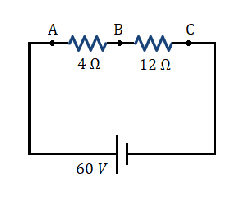
\includegraphics[width=\textwidth]{series.eps}
            \caption{Series connection.}
        \end{minipage}
        \hfill
        \begin{minipage}[b]{0.4\textwidth}
            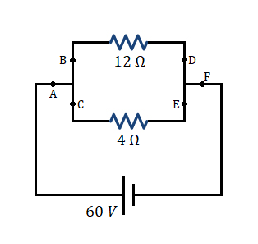
\includegraphics[width=\textwidth]{parallel.eps}
            \caption{Parallel connection.}
        \end{minipage}
    \end{figure}
    \begin{itemize}
        \item When connected in a series connection, resistances add together, i.e. $\boxed{R=\sum R_i}$ The same amount of current passes through both loads (calculated by calculating the effective resistance) but the voltage drops across each load. So,\newline$R=4+12=\boxed{16\text{ }\Omega}$, and \[I=I_A=I_B=I_C=\frac VR=\frac{60}{16}=\boxed{3.75\text{ A}}\]\[V_B=V_A-\Delta V=60-3.75\times4=\boxed{45\text{ V}}\]\[V_C=V_B-\Delta V=45-3.75\times12=\boxed{0\text{ V}}\implies\boxed{V_A>V_B>V_C}\] An \textit{ammeter} measures the current flowing through a wire and is always attached in series; its resistance is also made to be nearly 0 so the voltage does not change across its ends.
        \item When connected in a parallel connection, \[\boxed{\frac1R=\sum\frac1{R_i}}\] The ends of the parallel complex will be at the same voltage while the current will split across the branches. So, \[\frac1R=\frac1{12}+\frac14\implies R=\boxed{3\text{ }\Omega}\]\[V=V_A=V_B=V_C=\boxed{60\text{ V}}\text{ and }V_D=V_E=V_F=\boxed{0\text{ V}}\]\[I=I_A=I_F=\frac{60}3=\boxed{20\textrm{ A}}\]\[I_B=I_D=\frac V{R_1}=\frac{60}{12}=\boxed{5\textrm{ A}}\text{ and }I_C=I_E=\frac V{R_2}=\frac{60}4=I-I_B=\boxed{15\textrm{ A}}\] A \textit{voltmeter} measures the voltage across a wire and is always attached in parallel; its resistance is also made to be very high so nearly no current goes through it.
        \item \textbf{Important}: if at any point you get negative values for current (in the parallel connection case) or for voltage (in the series connection case), then remember that the resistances divide the current in inverse ratios of the whole and they divide the voltage in inverse ratios of the whole as well.
    \end{itemize}
    \subsubsection{Kirchhoff's Laws}
    \begin{enumerate}
        \item Junction Rule: essentially a statement of conservation of charge, it states that at a junction where multiple wires meet, the total amount of incoming current is equal to the total amount of outgoing current, i.e. $\boxed{I_\text{in}=I_\text{out}}$
        \item Loop Law: essentially a statement of conservation of energy, it states that the total voltage drop in any closed loop is 0, i.e. if current is flowing through an closed loop, then the amount of voltage drop will be recompensated by a battery or another device or $\boxed{\sum V_i=0}$
    \end{enumerate}
    \begin{figure}[H]
        \centering
        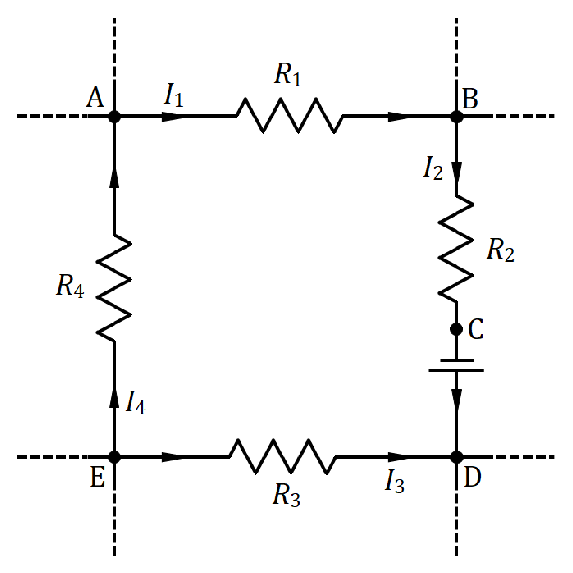
\includegraphics[scale=.75]{kirchhoff.eps}
        \caption{Closed loop of Kirchhoff's 2$^\text{nd}$ law.}
    \end{figure}
    \begin{itemize}
        Following the loop from point $A$ with voltage $\left(V_A\right)$ around the loop clockwise, we see,
        \begin{align*}
            \underbrace{\underbrace{\underbrace{\underbrace{\underbrace{V_A-I_1R_1}_{\text{Across resistor }1}-I_2R_2}_{\text{Across resistor }2}+\mathcal E}_{\text{Across battery}}+I_3R_3}_{\text{Across resistor }3}-I_4R_4}_{\text{Across resistor }4}=V_A
        \end{align*}
        Clearly the $V_A$ will cancel on both sides leaving the net voltage change to equal 0. \textit{This} is the statement of Kirchhoff's 2$^\text{nd}$ Law. And of course, the Junction Rule still holds as the algebraic sum of the current passing through points $A$, $B$, $D$, and $E$ is 0 as well.
    \end{itemize}
    \begin{itemize}
        \item \textbf{Important}: in a complicated circuit diagram, you can always combine points that have the same voltage. So if two distinct points 1 and 2 (say) have the same potential, you can make them to coincide and change the diagram appropriately. Another thing you can always do is make the length of a wire (with no electrical instrument on it) as long or as short as you want. So if points $A$ and $B$ are connected by a plain wire with nothing on it, they can be made to coincide.
    \end{itemize}
    \begin{figure}[H]
        \centering
        \begin{minipage}[b]{0.4\textwidth}
            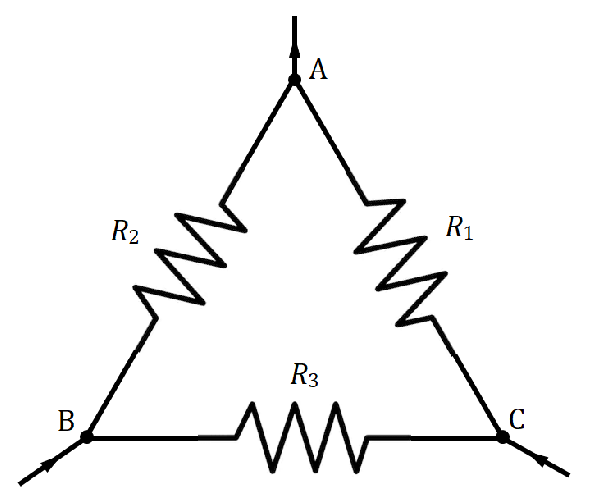
\includegraphics[width=\textwidth]{delta.eps}
            \caption{A delta configuration.}
        \end{minipage}
        \hfill
        \begin{minipage}[b]{0.4\textwidth}
            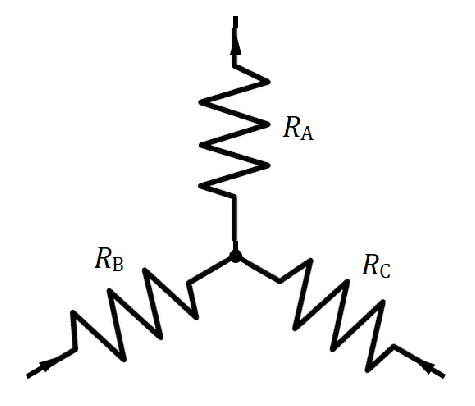
\includegraphics[width=\textwidth]{star.eps}
            \caption{A star configuration.}
        \end{minipage}
    \end{figure}
    \begin{itemize}
        \item While solving for equivalent resistance, there is something called the Star-Delta Method. So, if you have a structure like the one in Figure (11), called a Delta Formation, you can change to a Star Formation like the one in Figure (12). And the following are the resistances, \[R_A=\frac{R_1R_2}{R_1+R_2+R_3}\]\[R_B=\frac{R_2R_3}{R_1+R_2+R_3}\]\[R_C=\frac{R_1R_3}{R_1+R_2+R_3}\]
        \item To solve a complicated resistance structure, you can use symmetry to cut it into identical parts which may be easier to solve individually, and then they can be taken to be in series. Any resistances must be cut perpendicular to their connect and not paralell and these resistances are effectly halved. Symmetry in general is very important to physics and it can help reduce the mathematics dramatically.\footnote[1]{Check out Noether's Theorem (full disclosure: has \textit{nothing} to do with USAPhO):\\\url{https://en.wikipedia.org/wiki/Noether\%27s_theorem}}
        \item For batteries connected in series, the equivalent battery has an emf which is the \textit{algebraic} sum of the emfs of the individual batteries, i.e. $\boxed{\mathcal E=\sum\mathcal E_i}$ The direction for current is the direction for which $\mathcal E_i$ will be positive and it will be negative otherwise. The internal resistances of the batteries also add but for that, no sign needs to be taken into account.
        \item For batteries connected in parallel, their emfs add in a weighted average of the internal resistances' reciprocals, i.e.\[\boxed{\mathcal E=\frac{\sum\frac{\mathcal E_i}{r_i}}{\sum\frac1{r_i}}}\] The internal resistances add reciprocals as always, and the emfs need to be taken with appropriate signs as well.
    \end{itemize}
    \subsubsection{Capacitors}
    \quad A capacitor is a device that stores electrical energy to be released; however, \textit{unlike} a battery, the energy release is not slow and contained, but instantaneous.
    \begin{itemize}
        \item In a capacitor, the higher the voltage applied between the plates, the higher the charge that develops on the surfaces of the plates. Thus, $q\propto V\implies\boxed{q=CV}$ Here $C$ is known as the \textit{capacitance} of the capacitor and it's measured in \textit{farads} (F).
        \item \textbf{Important}: to find the capacitance of an arbitrary set-up, there a few steps to follow:
        \begin{enumerate}
            \item Assign charge $q$ to one surface and $-q$ to the other.
            \item Calculate $\vec{\mathbf E}$ between the two conductors using Gauss' Law.
            \item Calculate $|\Delta V|$ from the electric field calculated in step 2.
            \item Substitute the value of $\Delta V$ into $C=\dfrac q{|\Delta V|}$
        \end{enumerate}
        \item Using the method above, the capacitance for a parallel-plate capacitor with area $A$, and separation $d$ is given by, \[C_\parallel=\frac{\varepsilon A}d\]
        \item The capacitance of a spherical capacitor (with inner spherical radius $a$ and outer spherical radius $b$) is, \[C_\text{sphere}=\frac{4\pi\varepsilon ab}{\left(b-a\right)}=\frac{ab}{k\left(b-a\right)}\]
        \item The capacitance of a cylindrical capacitor (with inner cylindrical radius $a$, outer cylindrical radius $b$, and height $h$) is, \[C_\text{cylinder}=\frac{2\pi\varepsilon h}{\ln\frac ba}=\frac{h}{2k\ln\frac ba}\]
        \item To find the force of attraction on one plate of a parallel-plate capacitor of area $A$ simply multiply the charge of a plate by the electric field produced by the other plate. The net electric field between the plates is $\sfrac{q}{\varepsilon A}$, thus dividing it by two gives us the electric field to to plate 1 (positively charged). The force on plate 2 is then simply \[F_2=q_2E_1=-\frac{q^2}{2\varepsilon A}\] This force is felt by both plates and the negative sign denotes that it is an attractive force. Note that the force is independent of the separation, thus bringing the plates closer together of farther apart does not affect the force on the plates.
        \item \textbf{Important}: energy stored in a capacitor can be found by simply multiplying the attractive force on the plate by the separation of the capacitor, i.e. \[U_\textbf{capacitor}=\frac{q^2d}{2\varepsilon A}\implies\boxed{U_\textbf{capacitor}=\frac{q^2}{2C}=\frac12CV^2=\frac12qV}\] Note that the energy is positive since the work done was negative and potential energy is defined as the negative of the work done.
        \item To find the energy density in an electric field, we simply use a capacitor. We know that the energy stores in a capacitor is $U=CV^2/2$. Substituing $C=\sfrac{\varepsilon A}d$ and $V=Ed$, we get \[U=\frac12\varepsilon AdE^2\implies\frac U{Ad}=\rho_E=\frac12\varepsilon E^2\]
        \item If some capacitors are connected in series (where the capacitance of the $i^\text{th}$ capacitor is $C_i$) to a battery that delivers a voltage of $V$, then each capacitor will experience a potential drop across its terminals. The sum of these potential drops must equal $V$, thus, \[V=\sum V_i\implies\frac qC=\sum\frac q{C_i}\implies\boxed{\frac1C=\sum\frac1{C_i}}\] where $q$ is the charge provided to the first capacitor (which, in turn, charges \textit{every} capacitor with charge $q$).
        \item If some capacitors are connected in parallel (where the capacitance of the $i^\text{th}$ capacitor is $C_i$) to a battery that delivers a voltage of $V$, then each capacitor will experience the same voltage; however, the total charge the battery sends $q$ will be split among the capacitors, thus, \[q=\sum q_i\implies CV=\sum C_iV\implies\boxed{C=\sum C_i}\]
        \item A trick to remember while solving for equivalent capacitance when a bunch of metal sheets are given in complex connection, you can replace any plate which has only 1 surface in use by a symbol like $\perp$ and any plate where both surfaces are being used by an $\mathcal I$.
        \item Remember that in a complex circuit of capacitors, there will be a few "isolated elements" which will have $q_\text{net}=0$, and they can help you come up with nother equation to add to your system to solve later.
        \item To increase the capacitance of a capacitor, the region between the plates can be filled with a dielectric which increases the insulation between the two conductive plates. When placed under an external electric field, the atoms of a dielectric polarize and form their own opposing electric field, thus weakening the external electric field. This is measured by the dielectric constant and the \textit{electric susceptibility} of a material (it is the measure of how much a mertial will get polarized when placed in an external electric field; it is a dimensionless quantity, and is $\chi_E=\kappa-1)$, i.e. \[\kappa=\frac{E_0}{E_0-E_P}\implies E=\frac{E_0}\kappa\] Here $E_P$ is the electric field created by the dielectric. Inside a conductor, the net electric field is 0, i.e. $E_0=E_P\implies\kappa_\text{conductor}=\infty$; also, $\kappa_\text{vacuum}=1$. Integrating the above equation, we get \[V=\frac{V_0}{\kappa}\implies C=\kappa C_0\]
        \item Above a certain value of $E$, the polarization of the dielectric will become extreme enough to detach the electrons from the nuclei (effectively creating a plasma) and this is called dielectric breakdown.
        \item As soon as a battery is attached to a dielectric capacitor, the voltage is again increased to $V$ as the battery sends some extra charge to change the previous charge of $q$ to $\kappa q$. The electric field is again trestored to its original value, and the capacitance is left undisturbed. Now, even if the battery is disconnected, the charge will not change, and thus the system's properties will remain the same.
        \item If there are $n$ dielectric slabs of thicknesses $x_1,x_2,\dots,x_n$ and dielectric constants $\kappa_1,\kappa_2,\dots,\kappa_n$ between the plates of a capacitor separated by a distance $d$, then the capacitance becomes \[\boxed{C=\frac{\varepsilon A}{d-\sum x_i+\sum\frac{x_i}{\kappa_i}}}\] Note that this is essentially like taking away the thickness of a single slab and ``replacing" it with a thickness divided by the dielectric constant. Also note that $\varepsilon$ is the absolute permitivitty of the \textit{environment} and not that of any particular slab.
        \item When a dielectric is filled inside a capacitor, a net charge can also be induced in the dielectric. We already know that $E_0-E_P=E_0/\kappa$, and substituting $E_0=\sfrac q{\varepsilon A}$ and $E_P=\sfrac{q_P}{\varepsilon A}$, we get,\[\frac q{\varepsilon A}-\frac{q_P}{\varepsilon A}=\frac q{\kappa\varepsilon A}\implies\boxed{q_P=q\left(1-\frac1\kappa\right)}\] Thus the net charge on either plates can be taken to be $\boxed{q-q_P=\dfrac q\kappa}$
    \end{itemize}
    \subsection{Magnetism}
    \begin{itemize}
        \item When a wire carries current, at a certain point at some distance from the wire has no net electric field as the wire is neutral. The charges may be flowing \texit{through} the wire, but the wire itself is neutral. When a charge $q$ is placed t that point, it feels no net force, however when it is given some velocity, it does feel a net force. This is due to the \textit{magnetic} field produced by the wire and by experimentation, this force is found to be \[\boxed{\vec{\mathbf F}=q\vec{\mathbf v}\times\vec{\mathbf B}}\] Here $\vec{\mathbf B}$ is the magnetic field produced by the current, and $\vec{\mathbf v}$ is the velocity with which the charge is moved. If an electric field is also present, the net force (called the \textit{Lorentz Force}) is given by \[\boxed{\vec{\mathbf F}=q\left(\vec{\mathbf E}+\vec{\mathbf v}\times\vec{\mathbf B}\right)}\] The magnetic field is measured in N A$^{-1}$m$^{-1}$, which is called 1 tesla (T). Side note, $\vec{\mathbf B}$ is also called the magnetic flux density just like $\vec{\mathbf E}$ is the electric flux density, and just as electric flux density does \textit{not} mean the same thing as electric flux $\left(\Phi_E\right)$, the magnetic flux density does not mean the same thing as \textit{magnetic} flux $\left(\Phi_B\right)$.
        \item Use Fleming Left Hand rule to find the directions of the force due to a magentic field, the velocity, and the magnetic field. The thumb is $F$, the index finger is $B$, and the middle finger is $v$.
        \item Exactly as with electric flux, the magnetic flux is defined as the magnetic field through a given area and it's measured in Tm$^2$ or weber (Wb), i.e. \[\boxed{\Phi_B=\iint_S\vec{\mathbf B}\cdot\mathrm d\vec{\mathbf A}}\]
        \item The force on a wire crrying a current while being placed in an external magnetic field can be gotten by the firce on a single point charge, i.e. \[\vec{\mathbf F}=q\times\frac{\vec{\mathbf\ell}}t\times\vec{\mathbf B}\implies\boxed{\vec{\mathbf F}=\int I\vec{\mathbf B}\times\mathrm d\vec{\mathbf\ell}}\] Here, $\vec{\mathbf\ell}$ is the length vector of the wire, \textit{pointing in the direction of the current}. Note that if a specific wire configuration lies in a plane with a magnetic field perpecdicular to the plane, then the length is just replaced with the ``projected" length along the line joining the top and the bottom, as in the semi-circular wire example.
    \end{itemize}
    \subsubsection{Magnetic dipole}
    \begin{figure}[H]
        \centering
        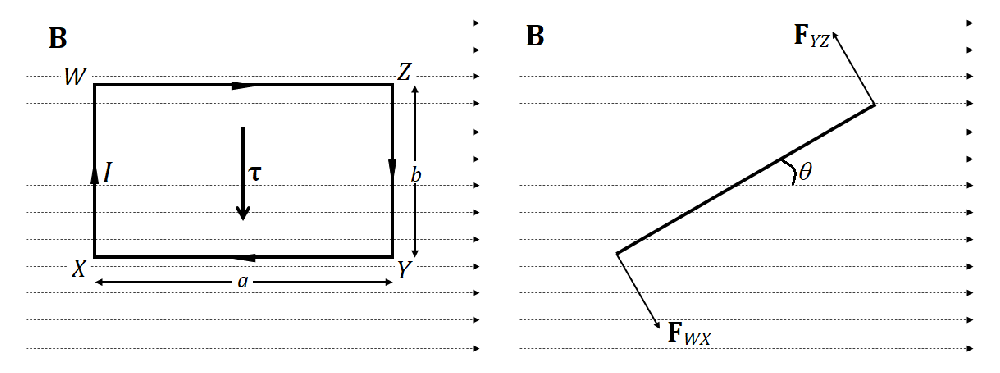
\includegraphics[scale=.9]{magneticdipole.eps}
        \caption{A closed loop in an external magnetic field.}
    \end{figure}
    \begin{itemize}
        \item If a closed loop $WXYZ$, carrying current $I$, inclined at an angle $\theta$ with the external magnetic field $\vec{\mathbf B}$ experiences a net torque $\vec{\mathbf \tau}$, the direction of which is shown in the Figure (13) on the left. This is because there is a net force on branch $YZ$ (the length of which is $b$), and on $WX$. There is 0 net force on $XY$ and $ZW$ since they are parallel to $\vec{\mathbf B}$. Now, $\vec{\mathbf F}_{YZ}=\vec{\mathbf F}_{WX}=I\vec{\mathbf b}\times\vec{\mathbf B}$, thus the torque is \[\vec{\mathbf \tau}=\frac {\vec{\mathbf a}}2\left(\vec{\mathbf F}_{YZ}+\vec{\mathbf F}_{WX}\right)=I\vec{\mathbf a}\times\vec{\mathbf b}\times\vec{\mathbf B}=I\vec{\mathbf A}\times\vec{\mathbf B}\] Now, this is valid if there's a single loop, but if there are multiple loops, this torque acts on each loop, thus the equation becomes $\vec{\mathbf \tau}=nI\vec{\mathbf A}\times\vec{\mathbf B}$ where $n$ is simply the number of loops. Now, defining $\vec{\mathbf m}_B$ to be $nI\vec{\mathbf A}$, and substituting this into the equation for torque, we get \[\boxed{\vec{\mathbf \tau}_B=\vec{\mathbf m}_B\times\vec{\mathbf B}}\] Comparing this to the equation, $\vec{\mathbf \tau}_E=\vec{\mathbf p}\times\vec{\mathbf E}$, $\vec{\mathbf m}_B$ is analogous to the electric dipole moment, thus, $\vec{\mathbf m}_B$ is called the \textit{magnetic dipole moment}.
        \item Just like with $\vec{\mathbf p}$, the potential energy held in the loop in a certain orientation is given by $\boxed{U_{B,\text{dipole}}=-\vec{\mathbf m}_B\cdot\vec{\mathbf B}}$ and just like the electric dipole moment is just the distance of the charges times the singular charge, $\boxed{\vec{\mathbf m}_B=2p\vec{\mathbf a}}$ where $2\vec{\mathbf a}$ is the distance vector \textit{from} the south \textit{to} the north pole, and $p$ here is the magnetic strength of one of the poles.
    \end{itemize}
    Exercise: do a couple examples, such as the magnetic dipole moment of a ring of charge $q$ rotating at $\omega$, and of a disk doing the same.
    \begin{itemize}
        \item There is an effect called the Hall effect which can help determine the sign of the charges in a conductor. Imagine a strip of metal with a current going down placed inside a magnetic field pointing into the metal (i.e. the direction is $\otimes$. By the way, to show a field pointing \textit{into} the paper, we use the symbol $\otimes$ representing the tail of an arrow, and we use the symbol $\odot$ to represent a field coming \textit{out of} the paper because it represents the tip of an arrowhead). If the charge is positive, it goes down, and if it's negative, it flows up. Either way, the magnetic field will cause the charges to drift towards the right and there will be a potential difference between the right and left sides of the strip; this is the Hall effect. Clearly, as more charges accumulate at the right, the potential difference will increase, and create an electric field in the strip, i.e. $\vec{\mathbf E}\cdot\vec{\mathbf d}=\Delta V$ where $d$ is the width of the strip. Charges will stop drifting when \[\vec{\mathbf F}=q\vec{\mathbf E}+q\vec{\mathbf v}_D\times\vec{\mathbf B}=0\implies\vec{\mathbf E}=-\vec{\mathbf v}_D\times\vec{\mathbf B}\] By knowing the direction of $\vec{\mathbf v}_D$, the drift velocity of the charges, the type of charge can be known.
        \item Now, if a particle is introduced into a region with magnetic field point into the paper $\left(\odot\right)$ with a velocity that lies in the plane, then the velocity and the magnetic field will produce a force that also lies in the plane perpendicular to the velocity, i.e. the charge cannot leave the paper, and its velocity will remain perpendicular to the magnetic field. Thus, the particle will perform uniform circular motion. Using the concepts of uniform circular motion, the following values can be calculated: \[\boxed{a_C=\frac{qvB}m\textrm{ }\textrm{ }\textrm{ }\textrm{ }\omega=\frac{qB}m\textrm{ }\textrm{ }\textrm{ }\textrm{ }r=\frac{mv}{qB}}\] Here, $m$ is the mass of the charge, and $\omega$ has a special name, called \textit{cyclotron frequency}. Also note that these equation are valid for small velocities; up until now, we have not dealt with relativistic speed, however, in a practical cyclotron, the speed regularly get close to $c$, thus relativistic mass and time must be used.
    \end{itemize}
    \subsubsection{Biot-Savart Law}
    \begin{figure}[H]
        \centering
        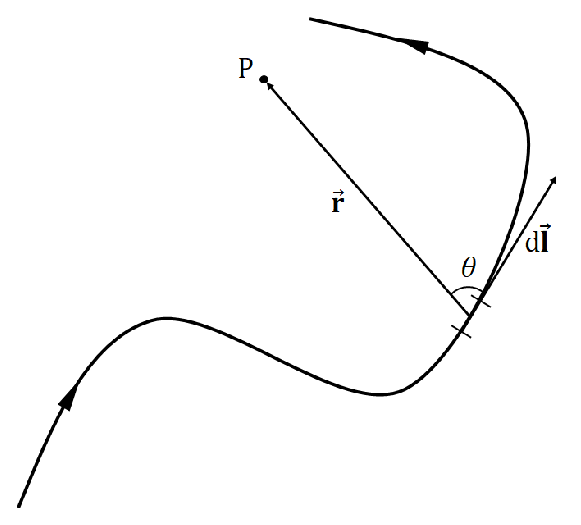
\includegraphics[scale=.6]{biot.eps}
        \caption{A wire carring a current, creating a magnetic field.}
    \end{figure}
    \begin{itemize}
        \item In the above figure, to find the magnetic field created by the wire carrying the current $I$, the Biot-Savart Law comes in handy. According to the law, the magnetic field at point $P$ is has an inverse square relationship with the small wire element $\mathrm d\vec{\mathbf\ell}$ and is directly proportional to the current in the wire, i.e. \[\mathrm d\vec{\mathbf B}\propto\frac{I\left(\mathrm dl\cdot r\sin\theta\right)}{r^3}\] Here, $r=\|\vec{\mathbf r}\|$ and the constant of proportionality will  not be a simple $k$, and just like with Coulomb's Law, we will write a more complex constant, \[\mathrm d\vec{\mathbf B}=\frac{\mu}{4\pi}\frac{I\left(\mathrm dl\cdot r\sin\theta\right)}{r^3}\implies\vec{\mathbf B}=\int\frac{I\mu}{4\pi}\frac{\mathrm d\vec{\mathbf\ell}\times\vec{\mathbf r}}{r^3}\implies\boxed{\vec{\mathbf B}=\frac{I\mu}{4\pi}\int\frac{\mathrm d\vec{\mathbf\ell}\times\hat{\mathbf r}}{r^2}}\] Here, $\mu$ is the absolute permeability of the surroundings, just as there is the absolute permittivity of the environment $\left(\varepsilon\right)$. Similarly, $\mu_0$ is the absolute permeability of free space or vacuum, and it's value was originally defined to be exactly $4\pi\times10^{-7}$ H m$^{-1}$; however after the 2019 redefinition of the SI system\footnote[2]{\label{secondfootnote}Check out wikipedia (full disclosure: has \textit{nothing} to do with USAPhO):\\\url{https://en.wikipedia.org/wiki/2019_redefinition_of_the_SI_base_units}}, it's no longer a defined constant, but an experimentally determined one. Moreover, $\mu=\mu_r\mu_0$ where $\mu_r$ is the relative magnetic permeability which is analogous to the dielectric constant $\kappa$.
        \item The magnetic susceptibility of a material is the measure of how much it will get magnetized when placed in an external magnetic field. It is a dimensionless quantity, and is $\chi_B=\mu_r-1$. It is analogous to the electric susceptibility of a material. \textbf{Important}: $\boxed{\mu_0\varepsilon_0c^2=1}$ where $c$ is the speed of light in a vacuum.
    \end{itemize}
    Exercise: do a couple examples, such as the magnetic field due to a ring of charge $q$ rotating at $\omega$ at the center, and of a disk doing the same.
    \begin{itemize}
        \item Two straight wires having current $I_1$ and $I_2$ flowing in the same direction and separated by a distance of $x$ will apply a force on each other sing the magnetic field produced by wire 1 will apply a force on the current of wire 2. The magnetic field from wire 1 at any point $L$ distance away will be \[B=\frac{\mu I_1}{2\pi x}\] And the force per unit length on the second wire by this magnetic field will be $I_2B$, or, \[\boxed{\frac{\mathrm dF}{\mathrm dl}=\frac{\mu I_1I_2}{2\pi x}}\] For the other wire, the force will be identical and this force will be \textit{attractive} for this specific case, but depending on the durection of the currents, a repulsive force can also be made. This was the pre-2019 definition of the ampere\footref{secondfootnote}.
    \end{itemize}
    \subsubsection{Amp\`ere's Law}\newline
    The circulation of the resultant magnetic field along a closed, planar curve is the product of $\mu$ and the total current crossing the area bounded by the closed curve.
    \begin{figure}[H]
        \centering
        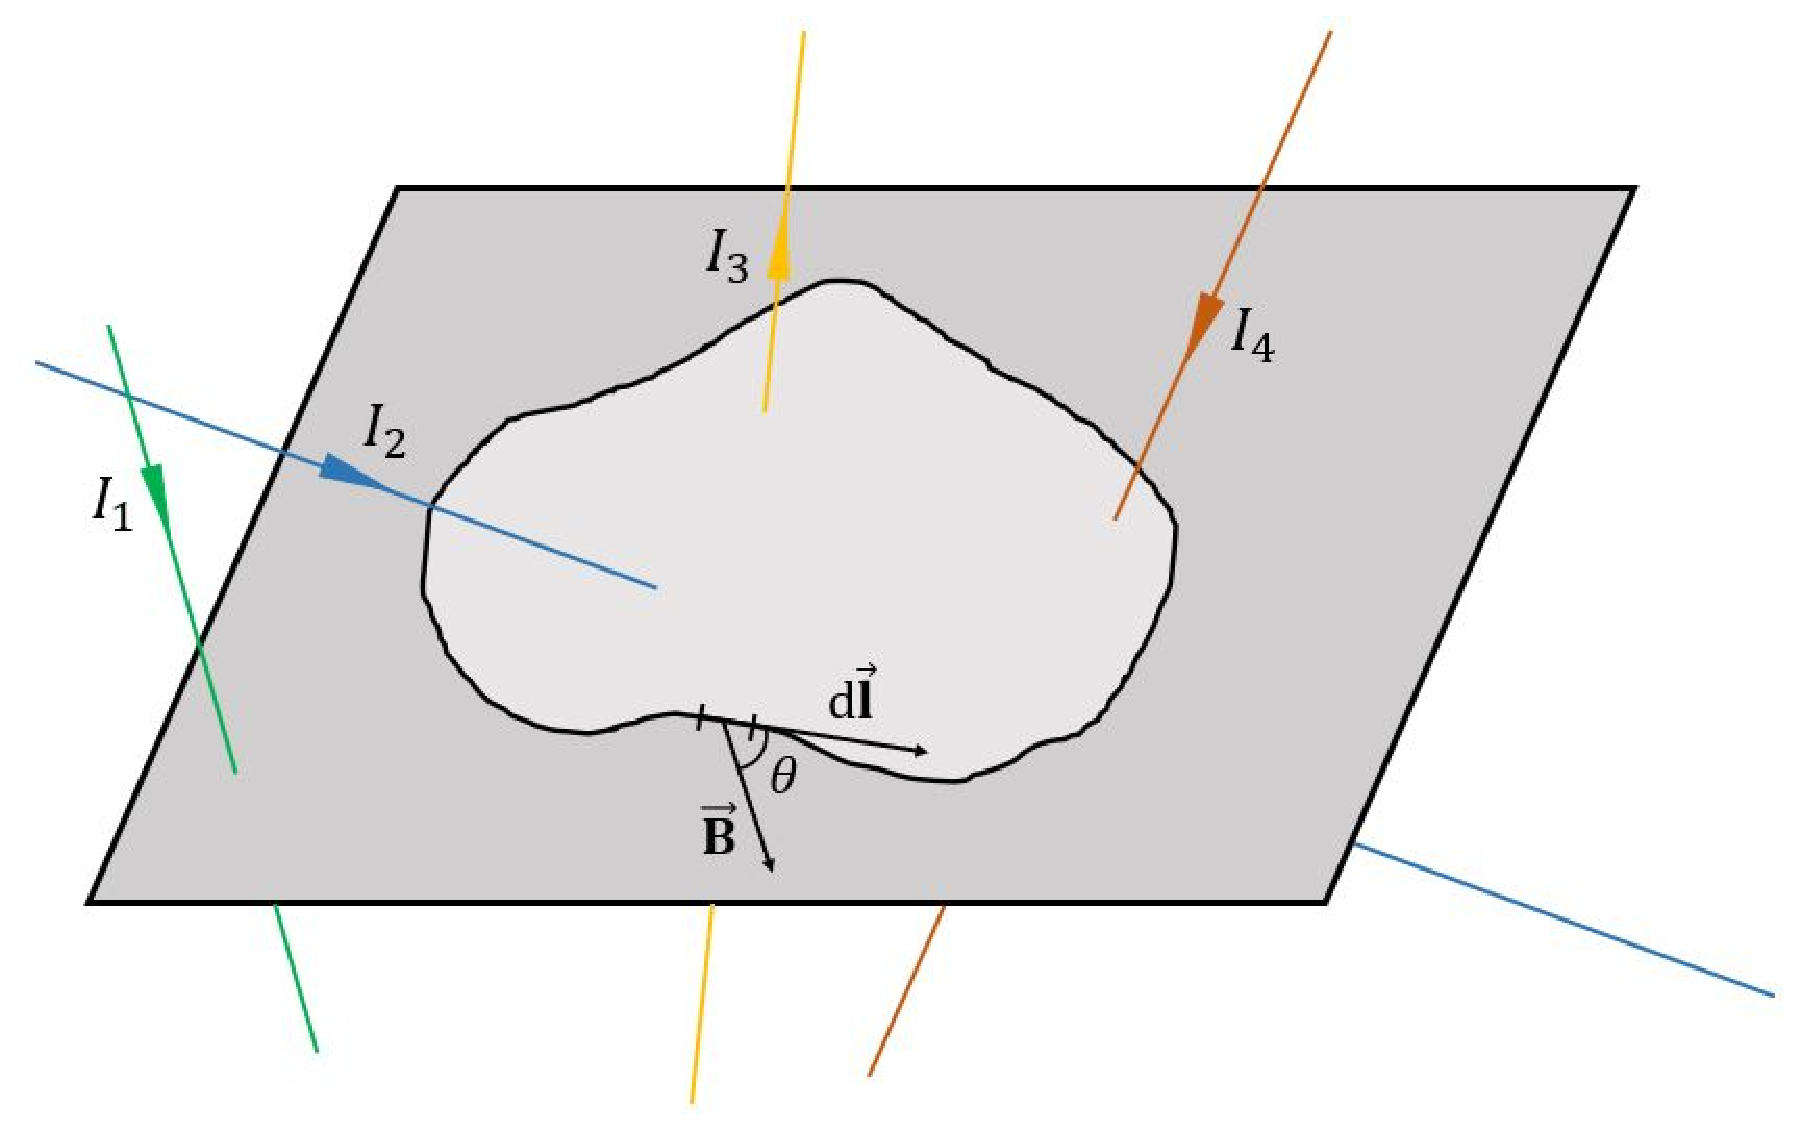
\includegraphics[scale=.45]{ampere.eps}
        \caption{A demonstration of Amp\`ere's Current Law.}
    \end{figure}
    Now, going counterclockwise around the plane surface bound by the closed loop shown above, the value of $\vec{\mathbf B}\cdot\mathrm d\vec{\mathbf\ell}$ integrated all around the closed loop, and it's value is just $\mu I_\text{enc}$; however using the right hand rule, the ``up" direction is found to be positive for $I$ and downward direction is negative. Thus, $\boxed{I_\text{enc}=I_3-I_2-I_4}$ Note that since $I_1$ is not passing through the surface, it does not contibute to $I_\text{enc}$. Thus, we get, \[\oint_{\partial \Sigma}\vec{\mathbf B}\cdot\mathrm d\vec{\mathbf\ell}=\mu I_\text{enc}=\mu\iint_\Sigma\vec{\mathbf J}\cdot\mathrm d\vec{\mathbf A}\] Now here's something that Amp\`ere could not explain. In a capacitor, as the charge builds up, the voltage (and thereby the electric field) increase over time. But there is no current flow between the plates of a capacitor; \textit{however}, a magnetic field is still produced! So, what Maxwell theorized was that a changing electric field (so a change in electric flux) is \textit{equivalent} to a current. This phenomenon is called \textit{\textbf{displacement current}} (as different from normal current called \textit{conduction current}) and it is this addition that completes Amp\`ere's Law; thus, we get, $\boxed{I_d=\varepsilon\dot\Phi_E}$ So to complete the law, we simply add this current to the total enclosed current, and we get \[\boxed{\oint_{\partial \Sigma}\vec{\mathbf B}\cdot\mathrm d\vec{\mathbf\ell}=\mu\left(\iint_\Sigma\vec{\mathbf J}\cdot\mathrm d\vec{\mathbf A}+\varepsilon\frac{\mathrm d}{\mathrm dt}\iint_\Sigma\vec{\mathbf E}\cdot\mathrm d\vec{\mathbf A}\right)}\implies\boxed{\vec{\mathbf\nabla}\times\vec{\mathbf B}=\mu\left(\vec{\mathbf J}+\varepsilon\frac{\partial\vec{\mathbf E}}{\partial t}\right)}\] So, if a variable electric field also exists across the surface, then its effect must be taken as an additional current. This is \textit{\textbf{Maxwell's Fourth Equation}}. Here subscript $\Sigma$ denotes that the surface over which to integrate on the right-hand side is enclosed by the curve over which to integrate on the left. Also, the del represents the ``curl" of the magnetic field rather than its gradient as we have seen it being used so far. We only dealt with it when we had to find if a force is conservative, and similarly, \[\vec{\mathbf \nabla}\times\vec{\mathbf B}=\begin{vmatrix} \mathbf{\hat i} & \mathbf{\hat j} & \mathbf{\hat k} \\\\\dfrac{\partial}{\partial x} & \dfrac{\partial}{\partial y} & \dfrac{\partial}{\partial z}\\\\B_x & B_y & B_z \\\end{vmatrix}=\mu\left(\vec{\mathbf J}+\varepsilon\frac{\partial\vec{\mathbf E}}{\partial t}\right)\]
    \begin{itemize}
        \item \textbf{Important}: Amp\`ere's Law is much like Gauss' Law in terms of its implementation. It is useless if used on a complex curve, thus only symmetric curves are used whose closed integral is easy to calculate. Thus, analogous to how spheres are usually chosen for the implementation of Gauss' Law to allow for a constant electric field, usually circular curves are used, because by symmetry, the magnetic field must be the same at all points.
        \item \textbf{Solenoid and Toroid Magnetic Fields}
    \end{itemize}
    \begin{figure}[H]
        \centering
        \begin{minipage}[b]{0.55\textwidth}
            \includegraphics[width=\textwidth]{solenoid.eps}
            \caption{A solenoid and its magnetic field.}
        \end{minipage}
        \hfill
        \begin{minipage}[b]{0.3\textwidth}
            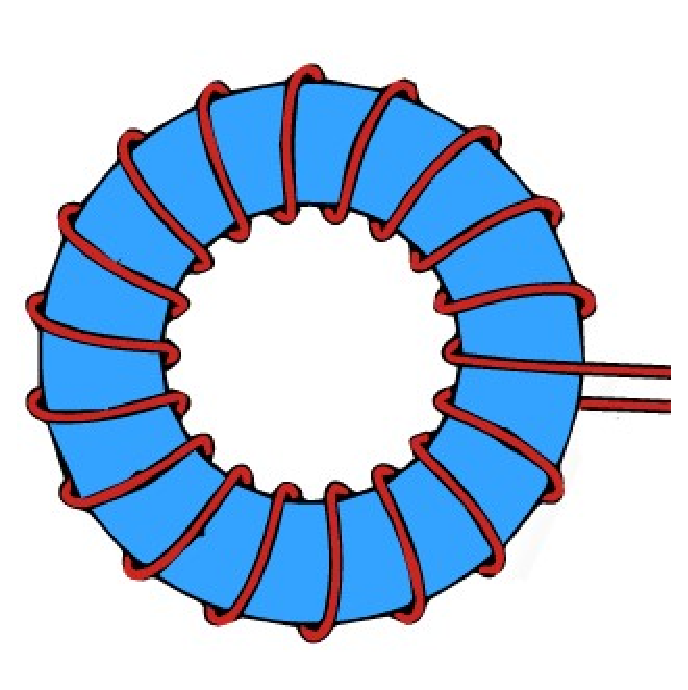
\includegraphics[width=\textwidth]{toroid.eps}
            \caption{A toroid.}
        \end{minipage}
    \end{figure}
    \begin{itemize}
        \item The magnetic field outside a solenoid is approximately 0 as the closely spaced loops cancel the magnetic field of each other outside the solenoid, and they increase the magnetic field inside the solenoid which is constant througout the inside as shown in Figure (16). If a solenoid has a $n$ turns per unit length, then the magnetic field inside the solenoid can be calculated using Amp\`ere's Law. In the Amp\`erian loop shown, the top segment and the top halves of the left and right segments will have 0 magnetic field. The bottom-halves of the left and right segments are perpendicular to the Amp\`erian loop, thus $\vec{\mathbf B}\cdot\mathrm d\vec{\mathbf\ell}=0$. For the bottom half, the magnetic field is $Bl$ and the enclosed current is simply, $nlI$. Thus, the magnetic field becomes \[Bl=\mu nlI\implies\boxed{B=\mu nI}\]
        \item Similar to a solenoid, a toroid will have nearly 0 magnetic field outside the toroid and inside the toroid, the magnetic field will be constant all around, by symmetry, but it will vary with radius. If the toroid has $N$ turns, then taking a concentric Amp\`erian circle with radius $R$, then the magnetic field can be easily calculated. It is simply \[B\oint_C\mathrm dl=\mu NI\implies\boxed{B=\frac{\mu NI}{2\pi R}}\]
    \end{itemize}
    \subsection{Electromagnetic Induction}
    \subsubsection{Faraday's Law}\newline
    Whenever there is a change in the magnetic flux through the area bounded by a closed, conducting loop, an emf is induced in the loop; this phenomenon is known as \textit{electromagnetic induction} (EMI).
    \begin{itemize}
        \item As the magnetic flux through a loop changes in some time, then an emf generates to oppose this effect, and this generate a current in the wire, i.e. $\boxed{\mathcal E=-\dot\Phi_B}$ The negative sign shows that $\mathcal E$ is generated to \textit{oppose} the magnetic flux change. Since the emf is simply the voltage produced, Faraday's Law can be re-written in another form, i.e. \[\boxed{\oint_{\partial\Sigma}\vec{\mathbf E}\cdot\mathrm d\vec{\mathbf \ell}=-\frac{\mathrm d}{\mathrm dt}\iint_\Sigma\vec{\mathbf B}\cdot\mathrm d\vec{\mathbf A}}\implies\boxed{\vec{\mathbf\nabla}\times\vec{\mathbf E}=-\frac{\partial\vec{\mathbf B}}{\partial t}}\] This result is \textbf{\textit{Maxwell's Third Equation}}.
        \item So, what happens is that when a magnetic flux changes through a closed loop, it generates a an emf in the wire so that the wire's produced magnetic field (cause by the induced current) opposes the external magnetic field in direction and magnitude; this is called \textbf{\textit{Lenz's Law}} and it helps you find the direction of the induced current in the wire loop. So if the magnetic flux decreases, the induced current will be such that it increases the flux by generating a magnetic field that points in the direction of the external magnetic field.
        \item Lenz's Law is an example of energy conservation. Consider a rectangular circuit (of length $\ell$) moving to the right (along its width) with a velocity $v$ and it enters a magnetic field which points into the plane $\left(\otimes\right)$. There will be an induced emf in the circuit, $\mathcal E=Bv\ell$, which will induce a current in the wire, $I=\mathcal E/R$ where $R$ is the circuit's resistance. This wire will experience a force $F=I\ell B$ (as it has a current flowing while in the presence of an external magnetic force) and this force will point in the direction \textit{opposite} to that of velocity. Thus, the magnetic field will slow the circuit down because it came in with a certain kinetic energy and as the current uses energy to move, it will draw this energy from the magnetic field, which will in turn draw it from the kinetic energy of the circuit (since the magnetic field must remain constant). Thus, the total energy of the system is conserved; \textit{this} is Lenz's Law.
        \item A generator is a device that converts mechanicl energy into electrical eneryg. It consists of a loop in a constant magnetic field. By some mechanical method, the loops is rotating with a constant angular frequency and the resulting induced $\mathcal E$ drives current; however the direction of the current changes direction as the flux increases, then decreases, and then increases again. Thus, this is hte generation of alternating current. Let $N$ loops have an area $A$, angular frequency $\omega$, placed in a constant external magnetic field $B$. Then, \[\mathcal E=-\dot\Phi_B=-\frac{\mathrm d}{\mathrm dt}\left[NAB\cos\left(\omega t\right)\right]=NAB\omega\sin\left(\omega t\right)\implies\boxed{I=\frac{NAB\omega}R\sin\left(\omega t\right)}\] Thus, the result yields that $I\propto\sin t$, and this is the definition of an alternating current. To find the power generated in a generator, simply use $P=\mathcal EI$, i.e. \[\boxed{P=\frac{\left(NAB\omega\right)^2}R\sin^2\left(\omega t\right)}\]
        \item The electric field induced by Faraday's Law is non-conservative in nature since as a charge goes around the loop, it gains kinetic energy and the energy by an electric field should be 0; this means that the concept of voltage does not apply since it is energy per unit charge, but after going around in a loop, the work done is non-zero, and so voltage from a point to the \textit{same} point is also non-zero which is invalid.
    \end{itemize}
    \subsubsection{Inductance and Inductors}\newline
    It is the ability of a circuit to resist a change in the current flowing through it
    \begin{itemize}
        \item Imagine a circular loop of wire is hooked up to a battery and a variable resistor whose value can be changed. Now, due to the current, a magnetic field will be produced in the area of the loop of the wire (Biot-Savart Law) and upon changing the resistance, the current in the wire will change which will change the magnetic field; \textit{however}, this change in magnetic flux will induce another current in the loop (in accordance to Faraday's Law) and depending on the direction, it could \textit{either} support the original flowing current, or go against it; this is phenomenon is called inductance. Clearly, the change in magnetic flux will depend on the original current , i.e. \[\Phi_B\propto-I\implies\Phi_B=-LI\implies\boxed{\mathcal E=-L\dot I}\] Here $L$ is the inductance and the induced emf is called \textit{back emf}; also, $L$ is measured in henry (equal to Wb A$^{-1}$).
        \item The inductance of a component is a purely geometrical property, i.e. it depends only on the shape of the inductor and on nothing else. Take a solenoid as an example; suppose it has a radius $r$, length $\ell$, and has $n$ turns per unit length. Clearly, $\Phi_B=\vec{\mathbf B}\cdot\vec{\mathbf A}=\pi\mu nIr^2$ for each loop, and thus the total flux just becomes $\Phi_B=\pi\mu n^2\ell Ir^2$. To find $L$, we simply differentiate to get, \[\dot\Phi_B=\pi\mu n^2\ell r^2\dot I\implies\boxed{L=\pi\mu n^2\ell r^2=\frac{\mu N^2A}\ell}\] Here, $N$ is the total number of turns in the solenoid, and $A$ is the cross-sectional area. Moreover, all the variables are geometrical properties of a solenoid, independent of the other electrical phenomenon!
    \end{itemize}
    \begin{figure}[H]
        \centering
        \begin{minipage}[b]{0.55\textwidth}.
        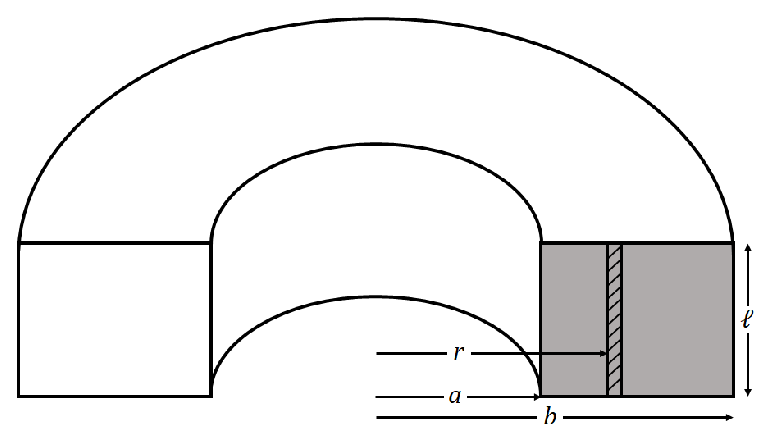
\includegraphics[width=\textwidth]{tor.eps}
        \caption{A square pseudo-toroid.}
        \end{minipage}
        \hfill
        \begin{minipage}[b]{0.4\textwidth}
            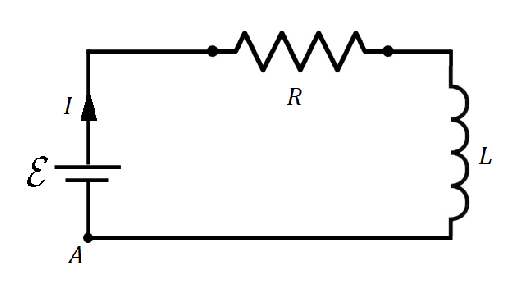
\includegraphics[width=\textwidth]{inductor.eps}
            \caption{A circuit with an inductor.}
        \end{minipage}
    \end{figure}
    \begin{itemize}
        \item To find the inductance of a toroid we revert to the magnetic field we derived for a toroid, but since it varies with the radius, we must integrate across the cross sectional area to find the flux; however, that particular integral is impossible to calculate analytically, and thus we must use a rectangular pseudo-toroid. Now, at a distance $r$, a slice of thickness $\mathrm dr$ will experience the flux, \[\mathrm d\Phi_B=\vec{\mathbf B}\cdot\mathrm d\vec{\mathbf A}=\frac{\mu NI}{2\pi r}\cdot \ell\mathrm dr\] Here, $N$ is the number of coils around the toroid each with current $I$ running through it. To find the total flux, we simply integrate (and multiply by $N$ since this flux is for 1 loop only), i.e. \[\Phi_B=\frac{\mu NI\ell}{2\pi}\int_a^b\frac{\mathrm dr}r=\frac{\mu N^2I\ell}{2\pi}\ln\frac ba\] Now, we differentiate with respect to time, to get, \[\dot\Phi_B=\frac{\mu N^2\ell\dot I}{2\pi}\ln\frac ba\implies L=\frac{\mu N^2\ell}{2\pi}\ln\frac ba\] Now, we can take an approximation for the $\ln$ function (as $x\to0$, the value of $\ln(1+x)\to x$), and get, \[L=\frac{\mu N^2\ell}{2\pi}\ln\left(1+\frac ba-1\right)\approx\frac{\mu N^2}{2\pi}\frac {\ell\left(b-a\right)}a\] Now, clearly this implies that $a\approx b$, and the numerator is simply the cross sectional area of the toroid, while the denominator is the ``length" of the toroid (\textit{\textbf{or more specifically}} the circumference of the circle with the radius to the toroid's center line, $R$), i.e. \[\boxed{L\approx\frac{\mu N^2A}{2\pi R}}\]
        \item If there's an inductor across the points $A$ and $B$, then the emf it induces is the same as the voltage difference across $A$ and $B$, thus $V_B-V_A=-L\dot I$. Now, if the current is increasing, i.e. $\dot I>0$, then the voltage difference turns out to be negative, or, $B$ is at a lower voltage than $A$. This means that the inductor is equivalent to a battery whose positive terminal points against the current, \textit{towards} point $A$ and whose emf is simply $\mathcal E$. If $\dot I<0$, then the inductor is equivalent to a battery that points in the direction of the current and strengthens it. Then, using an inductor as \textit{effectively} a battery, we can use Kirchhoff's Loop Law on the circuit.
        \item An inductor can also store energy (in the form of magnetic potential energy) just like a capacitor stores electrical potential energy. This is so because an inductor has a magnetic field and a field of any kind is simply an influence of energy at a point.\footnote[3]{Check out this video, it is really helpful: \url{https://youtu.be/KSylo01n5FY}}
        \item Applying Kirchhoff's 2$^\text{nd}$ Law in Figure (19) counterclockwise from point $A$, we get \[V_A+\mathcal E-IR-L\dot I=V_A\implies\mathcal E-IR-L\dot I=0\] Now, mutiplying by $I\mathrm dt$, we get \[\mathcal EI\mathrm dt-I^2R\mthrm dt=LI\mathrm dI\] Note that this is essentially energy balance. THe equation simply says that the cell provides an energy $\mathcal E\mathrm dq$ to the charges that flow through the battery, and the resistor takes an energy $I^2R\mathrm dt$ to move the current through it. Thus, the remaining energy must be stored in the inductor, and is simply $LI\mathrm dI$. Now, integrating on both sides, we get \[\int_0^t\mathcal EI-I^2R\mthrm dt=\int_0^ILI\mathrm dI\implies\mathcal EIt-I^2Rt=\boxed{U_\text{ind}=\frac12LI^2}\] Thus, that is the energy stored in an inductor at any point, and when the current is changed, the energy also changes. Energy density of a solenoid inductor is, \[u=\frac{U_\text{ind}}{\pi r^2\ell}=\frac{\mu n^2I^2}2\implies\boxed{u=\frac{B^2}{2\mu}}\] This formula is analogous to the formula we saw for the energy density of an electric field.
        \item As a battery is switched on, the inductor does not immediately acquire the current $I$ provide, but instead there is a more gradual growth of current. Going back to Figure (19) and the Kirchhoff equation we wrote, \[\mathcal E-IR=L\dot I\implies\frac{\mathrm dI}{\mathcal E-IR}=\frac{\mathrm dt}L\implies\int_0^I\frac{\mathrm dI}{\mathcal E-IR}=\int_0^t\frac{\mathrm dt}L\implies\boxed{I=\frac{\mathcal E}R-\frac{\mathcal E}Re^{-\frac RLt}}\] This is the growth of the current inside the inductor. Here, $\sfrac{\mathcal E}R$ is the maximum current that the inductor will hold (which will happen after an infinite amount of time). Here, the quantity $\sfrac LR$ is called the time constant (denoted by $\tau$), thus, the equation can be rewritten as \[I=I_\text{max}\left(1-e^{-\frac t\tau}\right)\implies\boxed{\mathcal E=\mathcal E_\text{max}\left(1-e^{-\frac t\tau}\right)}\] The growth for the emf is gotten by simply multiplying both sides by the resistance $R$.
        \item Now to find a decay function for the current, we revert to Figure (19) and replace the battery with a straight wire after a long time (after which the current in the inductor reaches its maximum). Re-writing Kirchhoff's Equation, we get $-IR=L\dot I$, and rewiting it we get, \[\frac{\mathrm dI}I=-\frac RL\mathrm dt\implies\int_{I_0}^I\frac{\mathrm dI}I=-\frac RL\int_0^t\mathrm dt\implies\boxed{I=I_0e^{-\frac RLt}}=I_0e^{-\frac t\tau}\] This is the decay function for the current where $I_0$ is the original current in the inductor and $\tau$ is again the time constant from the growth current derivation.
    \end{itemize}
    \begin{figure}[H]
        \centering
        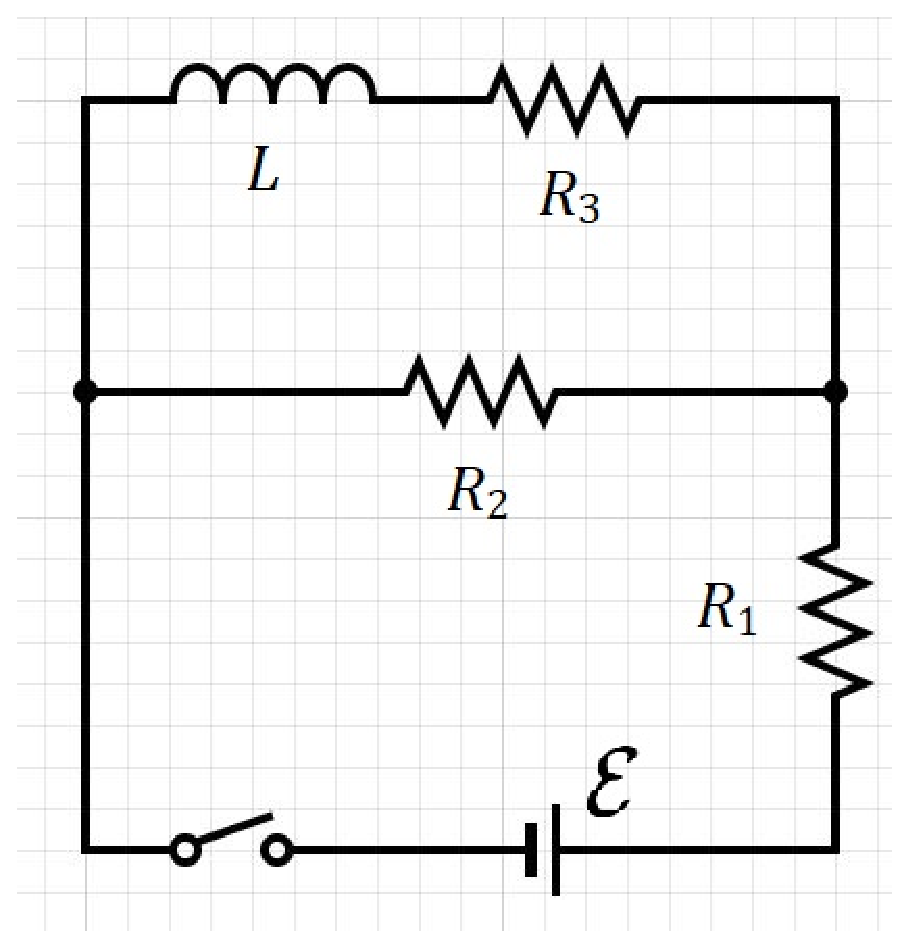
\includegraphics[scale=.3]{example.eps}
        \caption{A example circuit with an inductor.}
    \end{figure}
    Take the above circuit as an example. What will be the current in each branch just after the switch is closed? After a long time? What will be the heat dissipated by resistors 2 and 3 after $t$ time after the switch is opend (the switch is opened after a long time)?
    \begin{enumerate}[label=(\alph*)]
        \item Well, the inductor will let no current through after 0 time and hence the current in the upper branch will be 0. In the lower branch, the current is simply \[I=\frac{\mathcal E}{R_1+R_2}\]
        \item After a long time, when the inductor has had time to increase the current, it \textit{acts} like a straight wire, thus the circuit becomes a generic parallel-connection question.
        \item As soon as the switch is opened, the current will continue flowing in the upper loop, but the lower loop with have no current. Then, resistors 2 and 3, being in parallel, become equivalent to a single resistor with resistance $R=R_2+R_3$. The current in the inductor will be \[I=I_0e^{-\frac RLt}\] where $I_0$ is the current that can be found from the previous part. The energy sored in the inductor at time $t$ is simply \[U=\frac12LI^2=\frac12LI_0^2e^{-\frac{2R}Lt}\] Thus, the change in energy is equal to the heat the resistors dissipate, so, \[Q=\Delta U=\frac12LI_0^2e^{-\frac{2R}Lt}-\frac12LI_0^2=\boxed{\frac12LI_0^2\left(e^{-\frac{2\left(R_2+R_3\right)}Lt}-1\right)}\]
    \end{enumerate}
    \subsubsection{Gauss' Law for Magnetism}\newline
    Now, as you may have noticed, the magnetic field and electric field are similar to each other; however, there is one major difference: the exist no isolated magnetic monopoles. The simplest electric structure is simple a unit positive charge in free space, however, the simplest magnetic structure is a magnetic dipole. Upon cutting a magnetic in half, you do not result in a north magnetic and a south magnet. Instead, you get two small smaller magnets, each with its own north and south poles. Moreover, magnetic field lines are not produced from any pole and do not terminate at any pole either. They form only closed loops, even through a magnet where the magnetic field lines do not ``end" at either poles, but rather they continue on \textit{inside} the magnet as shown in Figure (21).
    \begin{figure}[H]
        \centering
        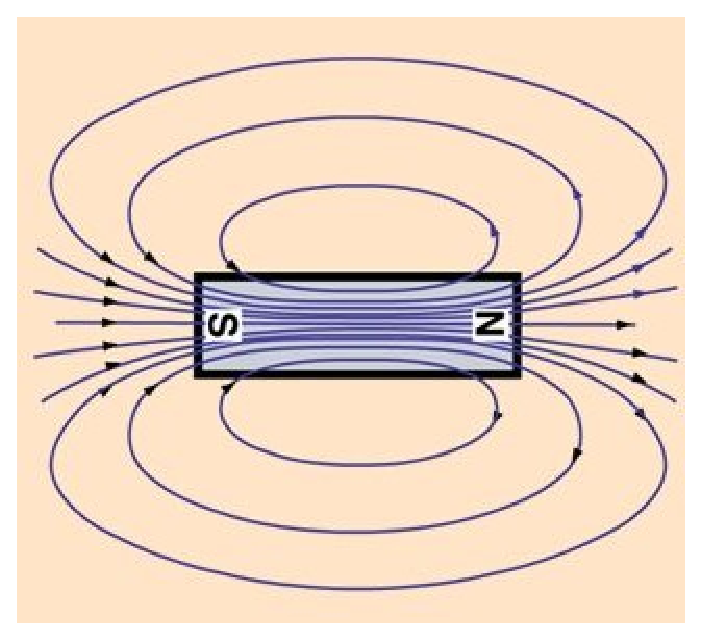
\includegraphics[scale=.5]{magnet.eps}
        \caption{Magnetic field lines through a magnet.}
    \end{figure}
    Magnetic field lines only ever ``begin" at infinity and if they do, they must also end at infinity because if it did not, then that would mean a south pole exists that has a bigger ``magnetic charge" than its accompanying north pole (since that north pole does not produce that extra magnetic field line). This would result in a net isolated magnetic pole, which is impossible. Thus, any magnetic field line must form a closed loop (having no beginning or end) or it must originate and end at infinity as well. Given these conditions, if one considers a Gaussian surface, every magnetic field line that enters the surface, must also exit, i.e. the \textit{net} magnetic flux through a Gaussian surface is 0. Thus, this law is equivalent to saying that an isolated magnetic monopole does not exist, and the following is \textit{\textbf{Maxwell's Second Equation}}: \[\Phi_{B,\text{net}}=\boxed{\oiint_{\partial\Omega}\vec{\mathbf B}\cdot\mathrm d\vec{\mathbf A}=0}\implies\boxed{\vec{\mathbf \nabla}\cdot\vec{\mathbf B}=0}\]
    \subsubsection{LC Circuits}\newline
    So gar we have worked with LR circuits (those with an inductor coupled with a passive resistor) and RC circuits (a passive resistor coupled with a capacitor). Now, we will study inductor-capacitor circuits.
    \begin{figure}[H]
        \centering
        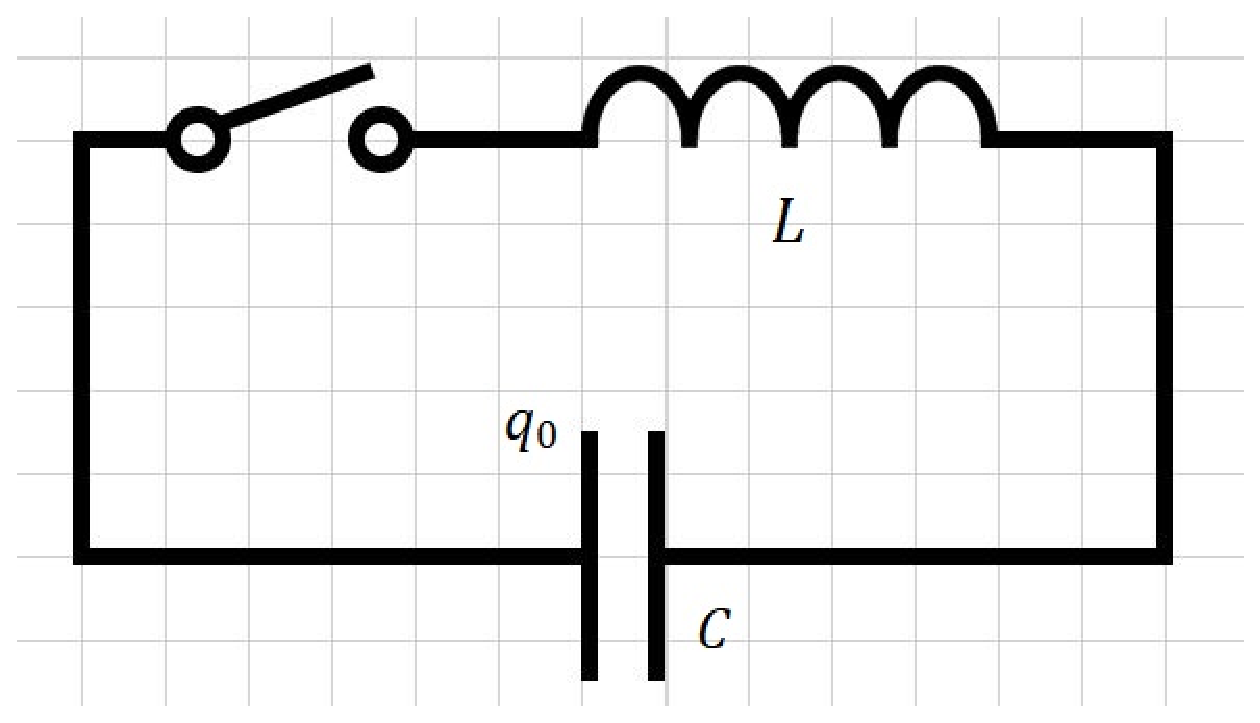
\includegraphics[scale=.35]{LC.eps}
        \caption{A generic LC circuit with a capacitor with charge $q_0$ and capacitance $C$.}
    \end{figure}
    \begin{itemize}
        \item In an LC circuit, the current performs oscillations and that makes this circuit special. If in Figure (22), the switch is closed at time $t=0$, then the current will start flowing from 0 and increase as the inductor lets more of the capacitor's current through it. We can write a Kirchhoff Equation from the bottom left corner counterclockwise: \[\frac{q_0}C-L\dot I=0\implies\frac{q_0}C=L\frac{\mathrm dI}{\mathrm dt}\implies\frac{q_0}{CL}=\frac{\mathrm d^2q}{\mathrm dt^2}\] Note that this is the equation of S.H.M. albeit the position here is replaced by the charge. Regardless, solving the equation gets us \[\boxed{q=q_0\cos\left(\frac t{\sqrt{CL}}+\phi\right)}\text{ }\text{, }\text{ }\text{ }\frac1{CL}=\omega^2\] Here, we use cosine because in S.H.M., there was a negative sign, and here this is not.
        \item Differentiating the above equation gets us $I=I_0\sin\left(\omega t\right)$. This is the condition for alternating current, i.e. an LC circuit produces an alternating current. This also shows that the current is maximum when the charge on the capacitor is 0, which makes sense as when the capacitor loses all of its charge, all the clost charge will be in motion, producing an AC.
        \item The time period of oscillation is $\boxed{T=2\pi\sqrt{LC}}$ This is twice the amount of time it takes for the charge to leave a plate and accumulate the charge on the other plate, i.e. for reversing the signs of the plates' charge. So, in time $\dfrac T2$, the plates' charges will exchange signs and after a whole time period passes, we will be back to the original situation again.
    \end{itemize}
    \begin{figure}[H]
        \centering
        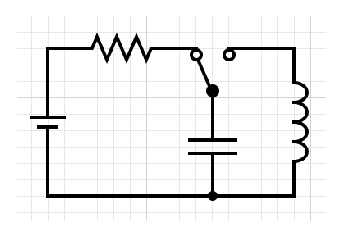
\includegraphics[scale=1.5]{ex.eps}
    \end{figure}
    \begin{itemize}
        \item The cell in the above circuit has an emf $\mathcal E$, and it has been connected to the capacitor (with capacitance $C$) for a long time; the inductor has an inductance $L$ and the resistor has a resistance $R$. Then, the switch is flipped at time $t=0$. Find
        \begin{enumerate}[label=(\alph*)]
            \item Maximum charge on the capacitor.
            \item Frequency of oscillation of the current.
            \item Maximum current in the inductor.
            \item Total energy as a function of time.
        \end{enumerate}
        \item Let the charge on the capacitor at some time $t$ ($t<0$) be $q$. Applying Kirchhoff's 2$^\text{nd}$ Law before the switch is flipped, we get \[\mathcal E-IR-\frac qC=0\implies\mathcal E=\frac{R\mathrm dq}{\mathrm dt}+\frac qC\implies\frac{\mathrm dq}{C\mathcal E-q}=\frac{\mathrm dt}{RC}\] Solving the differential equation, we get \[\int_0^q\frac{\mathrm dq}{C\mathcal E-q}=\int_0^t\frac{\mathrm dt}{RC}\implies\boxed{q=C\mathcal E\left(1-e^{-\frac t{RC}}\right)}\] This is the charge on the capacitor as a function of time. Now, since the capacitor had been hooked up to the cell for a long time, the charge was \[\lim_{t\to\infty}q=C\mathcal E\] This was the charge on the capacitor at time $t=0$ and after oscillations begin, this will remain its maximum charge.
        \item After the switch has been flipped, the charge will oscillate with a time period $T=2\pi\sqrt{CL}$. Now, to find the frequency of oscillations, we simply inverse it, to get \[\nu=\frac1{2\pi}\sqrt{\frac1{LC}}\]
        \item As we have already seen, when the charge on the capacitor is 0, the current in the inductor is at its maximum. This happens every time at $\sfrac T4$ and $\sfrac {3T}4$; thus pluggin in one of these values into the equation for current oscillation, we get \[I=q_0\omega\sin\left(\omega t\right)=\frac{C\mathcal E}{\sqrt{LC}}\sin\left(\frac{2\pi}T\frac T4\right)\implies\boxed{I_\text{max}=\mathcal E\sqrt{\frac CL}}\]
        \item When the charge on the capacitor is 0, the energy there is also 0. Thus, the total energy is just the energy in the inductor at that time (which happens to be the time when it has its maximum current). Thus, we get \[U_\text{max}=\frac12LI_\text{max}^2=\frac12C\mathcal E^2\]
    \end{itemize}
    \subsection{Alternating Current}
    \begin{itemize}
        \item As we have already seen, for a loop of wire rotating with angular velocity $\omega$ in a constant magnetic field, the magnetic flux through the loop is given by \[\Phi_B=\vec{\mathbf B}\cdot\vec{\mathbf A}=BA\cos\left(\omega t+\phi\right)\] Now the emf across the terminals of such a loop is given by Faraday's Law, i.e. \[\mathcal E=-\dot\Phi_B\implies\boxed{\mathcal E=-BA\omega\sin\left(\omega t+\phi\right)}\implies|\mathcal E|=\mathcal E_0\sin\left(\omega t+\phi\right)\] Thus, this proves that the emf must also alternate, and that makes sense as without emf alternating, the current cannot alternate because there will be nothing to drive it in the opposite direction. Dividing by the resistance, we get \[I=\frac{\mathcal E}R\implies\boxed{I=I_0\sin\left(\omega t+\phi\right)}\]
        \item The alternating current does not have to be sinusoidal in nature. Using the Fourier transform\footnote[4]{Check out the Fourier transform (full disclosure: has \textit{nothing} to do with USAPhO):\\\url{https://en.wikipedia.org/wiki/Fourier_transform}}, we can achieve any function from square waves to angular peaks as shown below.
    \end{itemize}
    \begin{figure}[H]
        \centering
        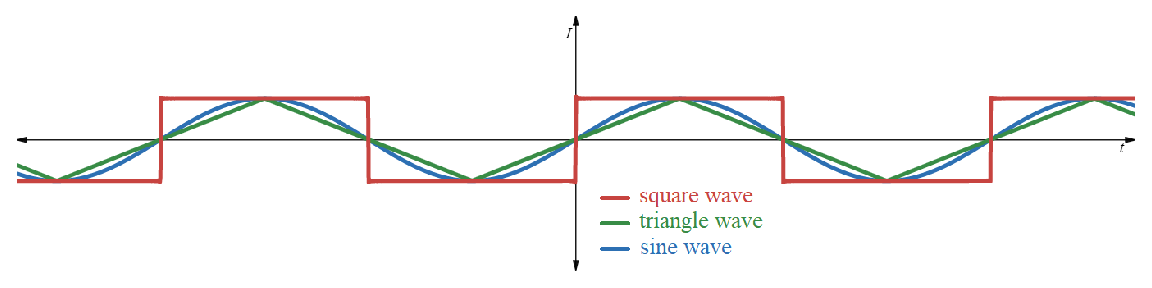
\includegraphics[scale=.66]{fourier.eps}
        \caption{These are the different types of ``waves" from the Fourier transform.}
    \end{figure}
    \begin{itemize}
        \item The average value of the current for a long time is clearly 0 since the integral over time is 0. Same holds true for 1 period, $T$. However, over half a period, the average value of the current is simply $I=2I_0/\pi$.
        \item There is also the RMS current associated with AC. This is simply the root mean-square of the current over a period. Thus, we get \[I_\text{RMS}=\sqrt{\left\langle I^2\right\rangle_0^T}=\sqrt{\frac{\int_0^TI_0^2\sin^2\left(\omega t\right)\mathrm dt}{\int_0^T\mathrm dt}}\implies\boxed{I_\text{RMS}=\frac{I_0}{\sqrt2}}\]
        \item When a capacitor is attached to an AC power supply, then the charge on the capcitor also follows a sinusoidal variation, i.e. \[\mathcal E=\frac qC\implies q=\mathcal E_0C\sin\left(\omega t\right)\implies \dot q=I=\mathcal E_0C\omega\cos\left(\omega t\right)\] Clearly, the current and the emf are out of phase by $\pi/2$, i.e. the emf of the AC source lags from the current by a phase of $\pi/2$. Moreover, $\mathcal E_0C\omega=I_0$ can be re-written as follows: \[I_0=\mathcal E_0C\omega=\frac{\mathcal E_0}{\frac1{C\omega}}=\frac{\mathcal E_0}{X_C}\implies\boxed{X_C=\frac1{C\omega}}\] Here, $X_C$ is the capacitive \textit{reactance} of the circuit. Reactance is simply the opposition of a circuit element to the flow of current due to its capacitance or inductance; capacitive reactance $\left(X_C\right)$ is measured in $\Omega$.
        \item When an inductor is hooked up to an AC power supply, then Kirchhoff's 2$^\text{nd}$ Law becomes, \[\mathcal E-L\frac{\mathrm dI}{\mathrm dt}=0\implies I=\int_0^t\frac{\mathcal E\mathrm dt}L\implies\boxed{I=-\frac{\mathcal E_0}{\omega L}\cos\left(\omega t\right)}\text{ }\text{, }\text{ }\text{ }\frac{\mathcal E_0}{\omega L}=\frac{\mathcal E_0}{X_L}=I_0\] Here $\left(X_L\right)$ is the inductive reactance of the inductor, and it is also measured in ohm. Also note that here, the current is also out of phase with the emf and the current now lags behind by a phase of $\pi/2$.
    \end{itemize}
    \subsubsection{Impedance}\newline
    \quad \textbf{It is the opposition to the current flow inside a circuit.}\footnote[5]{More resources: \url{https://en.wikipedia.org/wiki/Electrical_impedance} and\\\url{https://youtu.be/WmTlioVfS78}}
    \newline \quad Note that so far, we have seen two quantities, resistance and reactance, that are both described as ``opposition to current flow." Actually, they are only part of the big picture; the \textit{general} term for this phenomenon is impedance ($Z$).
    \newline \quad Now, since the current and emf are both sinusoidal functions, they can be re-written in terms of complex coefficients using Euler's formula \[\boxed{e^{\iota\theta}=\cos\theta+\iota\sin\theta}\] where $\iota$ is the imaginary unit ($i$ is not being used to avoid confusion with current; the resources listed below use $j$ as the imaginary unit for the same reason) and $\theta$ is the argument of the complex number. Now, the current and the emf can be re-written as \[I=\frac{I_0}2\left[e^{\iota\left(\omega t+\phi_I\right)}+e^{-\iota\left(\omega t+\phi_I\right)}\right]\implies\mathcal E=\frac{\mathcal E_0}2\left[e^{\iota\left(\omega t+\phi_{\mathcal E}\right)}+e^{-\iota\left(\omega t+\phi_{\mathcal E}\right)}\right]\]\[\therefore I=I_0\mathfrak R\left\{e^{\iota\left(\omega t+\phi_I\right)}\right\}\implies\mathcal E=\mathcal E_0\mathfrak R\left\{e^{\iota\left(\omega t+\phi_{\mathcal E_0}\right)}\right\}\] Now, the above formulae give the values of current and emf in terms of cosine, but that is a non-issue because all cosine functions can be written (with suitable phase differences) as sine functions. Likewise, we are also ignoring direction as magnitudes are of greater importance. So, both current and emf are scalar quantities and follow the law of superposition, just like forces; thus, to analyze the current of an AC circuit, we can analyze each complex part individually, and add the result. So, now that we are analyzing a more general case (of complex-valued current and emf), we introduce impedance rather than resistance; it simply takes over the analogous role in Ohm's Law, thus, \[Z=\frac{\mathcal E}I=\frac{\mathcal E_0e^{\iota\left(\omega t+\phi_{\mathcal E}\right)}}{I_0e^{\iota\left(\omega t+\phi_I\right)}}\implies\boxed{Z=\frac{\mathcal E_0}{I_0}e^{\iota\left(\phi_{\mathcal E}-\phi_I\right)}}\]
    \quad Now, we apply these tools to analyze pure AC resistive, capacitive, and inductive circuits again. Now, the above formula is actually the case for a simple resistor, so we already know the impedance due to a passive resistor. However, we also know that when attached to a resistor, both the voltage and the current are perfectly in phase, thus $\phi_{\mathcal E}=\phi_I$. This means the imaginary part of the formula is 0, and the impedance turns out to be a real number. This indicates that the \textbf{\textit{real part of the impedance is the resistance}}, or $\boxed{R=\mathfrak R\left\{Z\right\}}$
    \newline\quad In a pure capacitive AC circuit, the current leads by a phase of $\sfrac\pi2$, i.e. \[Z=\frac{\mathcal E_0}{I_0}e^{\iota\left(\phi_{\mathcal E}-\phi_I\right)}=\frac{\mathcal E_0}{I_0}e^{\iota\left(0-\frac\pi2\right)}=-\frac{\mathcal E_0}{I_0}\iota\] Now, in a capacitive circuit, $\sfrac{\mthcal E_0}{I_0}=X_C$, so we get $\boxed{Z=-X_C\iota}$ Thus, with a capacitor, the impedance is a purely imaginary quantity that is actually the capacitive reactance.
    \newline\quad Likewise, in a purely inductive circuit, the emf leads by a phase of $\sfrac\pi2$, i.e. \[Z=\frac{\mathcal E_0}{I_0}e^{\iota\left(\phi_{\mathcal E}-\phi_I\right)}=\frac{\mathcal E_0}{I_0}e^{\iota\left(\frac\pi2-0\right)}=\frac{\mathcal E_0}{I_0}\iota=X_L\iota\] So, we see the same result here, the impedance of a purely inductive circuit is a purely imaginary number, and is the inductive reactance of the inductor. So, this indicates that the \textbf{\textit{imaginary part of the impedance is the reactance}}, or $\boxed{X=\mathfrak I\left\{Z\right\}}$
    \newline\quad So, while solving problems, you make a \textit{phasor} just as we did in S.H.M. You find the resistance and that becomes a vector in the positive $x$-direction. Then, you find the capacitive reactance and that becomes a vector in the negative $y$-direction while the inductive reactance becomes a vector in the positive $y$-direction. The sum of these vectors (which is equivalent to adding complex numbers) gives us the impedance vector. Now, the impedance is not actually a vector; it is merely the sum of quantities (which also themselves are not vectors) in a phasor like shown below.
    \begin{figure}[H]
        \centering
        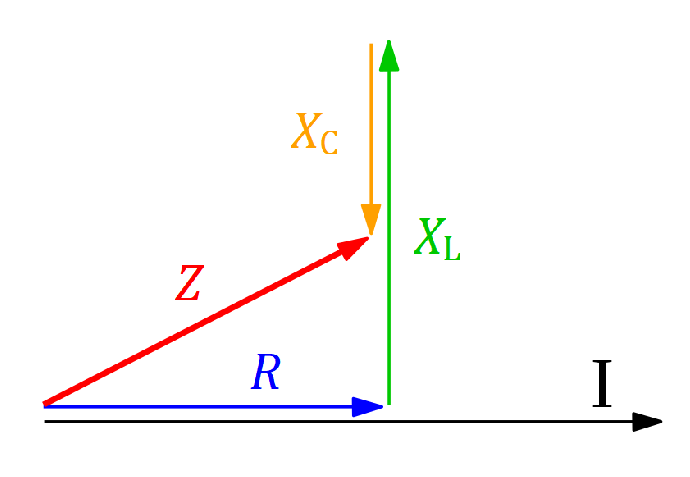
\includegraphics[scale=.66]{phasor.eps}
        \caption{This is an example of an electric phasor.}
    \end{figure}
    \textbf{Warning}: do not make the mistake of thinking that because we used the complex plane for this theory, that reactance or impedance are imaginary quantities. They are real, we just used a mathematical tool to find their values. It is more appropriate to say that impedance needs two numbers to fully describe, much like a point on the Cartesian plane. In fact, we could have used the Cartesian plane to arrive at the exact same conclusions. The purpose of using the complex plane is that Euler's formula allows us to work with exponential complex numbers which are easier.
    \quad So, the impedance can be written as a Cartesian complex number as $\boxed{Z=R+X\iota}$ where $R$ is the circuit's total resistance and $X$ is the total reactance. However, the complex number is not very useful, so we find the modulus of the impedance, i.e. \[|Z|=\sqrt{R^2+X^2}\] Then this value can be used as a ``resistance" for all AC problems; it is simply the resistance analogue for AC. It is measured in $\Omega$ and it adds in series just like resistance as well, i.e. \[\boxed{Z_\text{series}=\sum_{i=1}^nZ_i}\text{ }\text{ }\text{ }\boxed{\frac1{Z_\text{parallel}}=\sum_{i=1}^n\frac1{Z_i}}\] \blfootnote{The reciprocal of resistance is called conductance ($G)$; that of reactance is called susceptance ($B$), not to be confused with electric/magnetic \textit{susceptibility}; and that of impedance is called admittance ($Y$). They are related by the formula $\boxed{Y=G+B\iota}$ and are all measure in siemen (S).}
    \begin{itemize}
        \item Now, we can use these concepts to solve problems where capacitors, inductors, and resistors are attached together in an AC circuit. If, for example, you have a RC circuit with AC, then using Kirchhoff's Loop Law and using calculus is too tedious. Thus, we use the impedance. The emf is $\mathcal E=\mathcal E_0\sin\left(\omega t\right)$, and to find the equation for current, we get \[I=\frac{\mathcal E}Z=\frac{\mathcal E_0}{\sqrt{R^2+X_C^2}}\sin\left(\omega t+\phi\right)\] Here, $\phi$ is simply the phase difference of the current and emf (the $\phi_\mathcal{E}-\phi_I$ in the above explanation), so to find it, we simply find the complex argument of $Z$, or \[\phi=\boxed{\arg\left(Z\right)=\tan^{-1}\frac XR}=\tan^{-1}\frac{X_C}R\] Now, in competitions, this value will almost always turn out to be an easy multiple of $\pi$. So, the equation of the current becomes \[\boxed{I=\frac{\mathcal E_0}{\sqrt{R^2+X_C^2}}\sin\left(\omega t+\tan^{-1}\frac{X_C}R\right)}\]
        \item \textbf{Important}: the voltage drop across inductors, capacitors, and resistors also add in a phasor space, just as impedance does. So, if you have an AC source of peak voltage $100\sqrt2$ V, and the voltage drop across a resistor is 60 V, then the voltage drop across an inductor is given by \[V_\text{RMS}^2=V_R^2+V_L^2\implies10000=3600+V_L^2\implies V_L=80\text{ V}\]
    \end{itemize}
    \subsubsection{AC Resonance}
    \newline\quad Imagine a RLC circuit with an AC power source of emf $\mathcal E_0\sin\left(\omega t\right)$. Now, $I=\sfrac{\mathcal E}Z$, so to maximize current, we must minimize impedance, or \[Z=\sqrt{R^2+\left(X_L-X_C\right)^2}\implies\boxed{X_L=X_C}\] The above must hold because it maximizes the current and \textit{\textbf{this condition is called the condition of resonance of an AC circuit}}. Thus, the condition when the circuit is equivalent to a pure resistive circuit, is the resonance condition of that circuit. This means that, \[\omega L=\frac1{\omega C}\implies\boxed{\omega^2LC=1}\implies\arg\left(Z\right)=0\]
    \newline\quad The power in an AC circuit is given by \[P=\mathcal EI=\mathcal E_0\sin\left(\omega t\right)\cdot\frac{\mathcal E_0}Z\sin\left(\omega t+\phi\right)\implies\boxed{P=\frac{\mathcal E}Z\sin\left(\omega t+\phi\right)\sin\left(\omega t\right)}\] To find the average power, we take the average of this function, and we get \[\langle P\rangle=\frac{\mathcal E_0^2}{2Z}\cos\phi\implies\frac{\langle P\rangle}{\cos\phi}=\boxed{\frac{\langle P\rangle}{\cos\left[\arg\left(Z\right)\right]}=\frac{\mathcal E_\text{RMS}^2}Z=I_\text{RMS}^2Z=\mathcal E_\text{RMS}I_\text{RMS}}\]
    \section{Optics}
    \subsection{Geometrical Optics}\newline
    This is the the study of the behavior of light under reflections, refractions, etc.
    \subsubsection{Shadow Formation}\newline
    \quad There are four cases to consider here: a point light source, and a point object; a point light source, and an extended object; an extended light source, and a point object; and, and an extended light source, and an extended object; Here, cases 1-3 are simple, however case 4 is worth detailed analysis.
    \begin{figure}[H]
        \centering
        \includegraphics[scale=.6]{case4.eps}
        \caption{Case 4 has three variants as shown above.}
    \end{figure}
    \subsubsection{Reflection}
    \newline\quad Laws of reflection
    \begin{enumerate}
        \item The incident ray, the reflected ray, and the normal to the surface on the point of reflection all lie in the same plane.
        \item The angle of incidence and the angle of reflection are congruent, i.e. $\boxed{\angle \theta_i\cong\angle \theta_r}$
    \end{enumerate}
    \quad These laws are applicable for all smooth surfaces.
    \begin{itemize}
        \item If $\vec{\mathbf e}_i$ is the incident ray vector, and $\vec{\mathbf e}_r$ is the reflected ray vector, then the following holds: $\boxed{\vec{\mathbf e}_r=\vec{\mathbf e}_i-2\left(\vec{\mathbf e}_i\cdot\hat{\mathbf n}\right)\hat{\mathbf n}}$ Here $\hat{\mathbf n}$ is the unit vector along the normal.
        \item \textbf{Important}: while drawing diagrams, every point where two incidence rays intersect coincides with a point on the object and every point where two reflected rays intersect coincides with a point on the image. If two rays \textit{actually} intersect, the object/image is real, otherwise, the image is virtual.
        \item A spherical mirror is one which subtends some solid angle on the center of a sphere. The radius of curvature ($R_C$) is the radius of this sphere and the center of curvature (point $C$) is the center upon which the solid angle is subtended. The aperture ($A$) is the size of the opening of the mirror as shown below. The co-ordinate system to be used is also shown.
    \end{itemize}
    \begin{figure}[H]
        \centering
        \begin{minipage}[b]{0.49\textwidth}.
        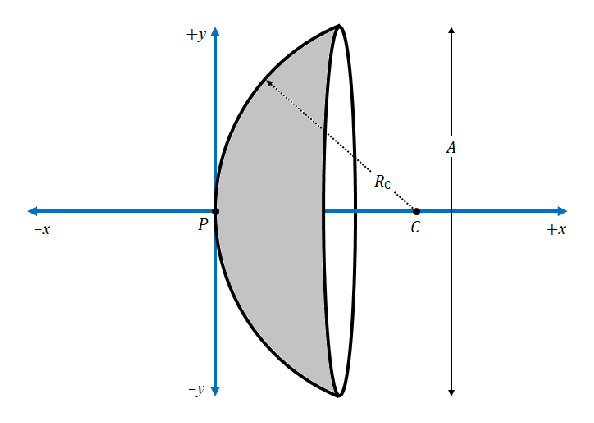
\includegraphics[width=\textwidth]{convexmirror.eps}
        \caption{A convex spherical mirror.}
        \end{minipage}
        \hfill
        \begin{minipage}[b]{0.49\textwidth}
            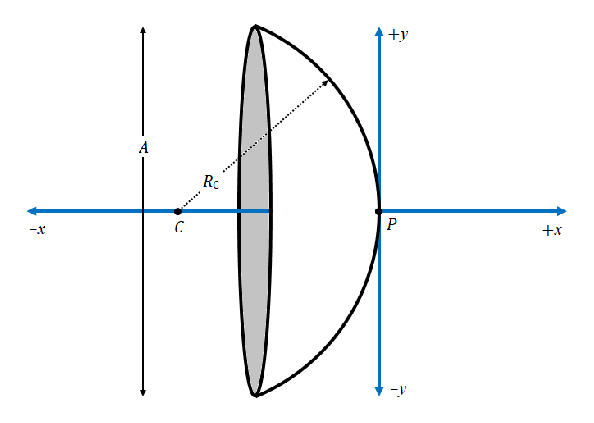
\includegraphics[width=\textwidth]{concavemirror.eps}
            \caption{A concave spherical mirror.}
        \end{minipage}
    \end{figure}
    \begin{itemize}
        \item In the above figures, the $x$-axis is also called the \textit{principal axis}. The radius of curvature can be found by using the formula given on the first page of this manuel. For small spherical mirrors, the aperture is effectively equal to the diameter of the sphere.
        \item The \textit{focus} is the point where a light beam, parallel to the principal axis, form a point image. For a spherical mirror with its center of curvature at point $C(x,0)$ will have its focus at the point $F(x/2,0)$. The distance between the focus and the pole is known as the \textit{focal length} of the mirror, and for spherical mirrors, the focal length ($f$) is $\boxed{R_C/2}$ if the mirror is taken to be small.
    \end{itemize}
    \quad\textbf{Concave Mirror}
    \begin{enumerate}
        \item \textit{Object between} $P$ \textit{and} $F$: if the object is within the focal length, the image formed is virtual (since the reflected rays \textit{produced} intersect), upright, and larger than the original object.
        \item \textit{Object on} $F$: if the object is on the focal point, the ``image" formed is at infinity (since the reflected rays are parallel).
        \item \textit{Object between} $F$ \textit{and} $C$: if the object is within the focal point and center of curvature, the image formed is real (since the reflected rays actually intersect), inverted, and larger than the original object.
        \item \textit{Object on} $C$: if the object is on the center of curvature, the image formed is real (since the reflected rays actually intersect), inverted, and the same size as the original object.
        \item \textit{Object beyond} $C$: if the object is farther than the radius of curvature, the image formed is real (since the reflected rays actually intersect), inverted, and smaller than the original object.
        \item \textit{Object at infinity}: if the object is infinitely far away, the ``image" formed will have 0 size, and be located at the focal point.
    \end{enumerate}
    \begin{figure}[H]
        \centering
        \begin{minipage}[b]{0.49\textwidth}.
        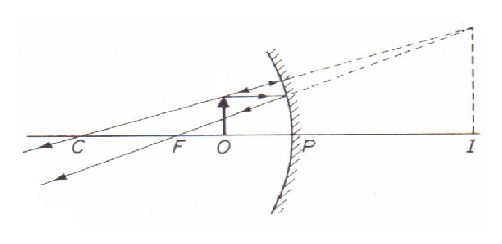
\includegraphics[width=\textwidth]{concave1.eps}
        \caption{\textit{Object between} $P$ \textit{and} $F$.}
        \end{minipage}
        \hfill
        \begin{minipage}[b]{0.49\textwidth}
            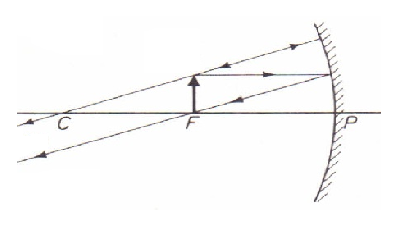
\includegraphics[width=\textwidth]{concave2.eps}
            \caption{\textit{Object on} $F$.}
        \end{minipage}
    \end{figure}
    \begin{figure}[H]
        \centering
        \begin{minipage}[b]{0.49\textwidth}.
        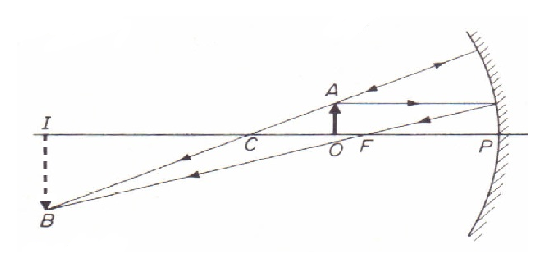
\includegraphics[width=\textwidth]{concave3.eps}
        \caption{\textit{Object between} $F$ \textit{and} $C$.}
        \end{minipage}
        \hfill
        \begin{minipage}[b]{0.49\textwidth}
            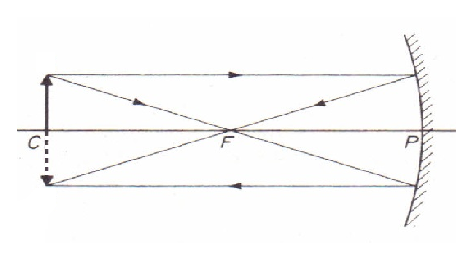
\includegraphics[width=\textwidth]{concave4.eps}
            \caption{\textit{Object on} $C$.}
        \end{minipage}
    \end{figure}
    \begin{figure}[H]
        \centering
        \begin{minipage}[b]{0.49\textwidth}.
        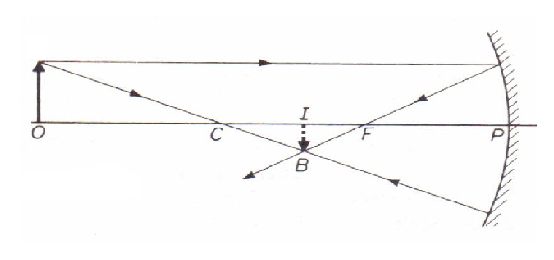
\includegraphics[width=\textwidth]{concave5.eps}
        \caption{\textit{Object beyond} $C$.}
        \end{minipage}
        \hfill
        \begin{minipage}[b]{0.49\textwidth}
            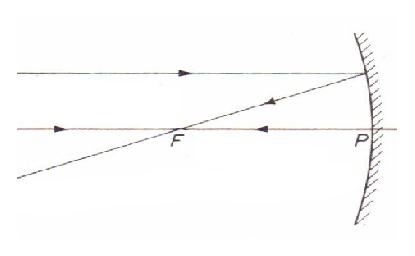
\includegraphics[width=\textwidth]{concave6.eps}
            \caption{\textit{Object at infinity}.}
        \end{minipage}
    \end{figure}
    \quad\textbf{Convex Mirror}
    \begin{enumerate}
        \item \textit{Object between} $P$ \textit{and infinity}: if the object is a finite distance away from the mirror, the image formed is between the pole and the focal point, and is virtual (since the reflected rays \textit{produced} intersect), inverted, and smaller than the original object.
        \item \textit{Object at infinity}: if the object is at infinity, then the ``image" formed will be a point at the focal point.
    \end{enumerate}
    \begin{itemize}
        \item The \textbf{Mirror Equation}\footnote[6]{Check out this video; it is a derivation: \url{https://youtu.be/OIkD1viOMWk}} is really helpful for doing calculations. If an object is a distance $u$ away from the pole of a mirror with focal length $f$, then the distance of the image from the pole ($v$) is given by \[\frac2{R_C}=\boxed{\frac1f=\frac1u+\frac1v}\]
        \item The magnification is also helpful while dealing with optics. The magnification of an optical instrument is simply the ratio of the height of the image $\left(h_i\right)$ and of the object $\left(h_o\right)$, or \[\boxed{M=\frac{h_i}{h_o}=-\frac vu}\] \textit{The sign conventions specified in} Figures (26) \textit{and} (27) \textit{must be followed for both magnification and the Mirror Equation}. A negative value of $M$ corresponds to a real image and a positive value implies a virtual image.
        \item
    \end{itemize}
    \quad\textbf{Convex Lens}
    \begin{enumerate}
        \item \textit{Object between} $P$ \textit{and} $F$: if the object is within the focal length, the image formed is virtual (since the reflected rays \textit{produced} intersect), upright, and larger than the original object.
        \item \textit{Object on} $F$: if the object is on the focal point, the ``image" formed is at infinity (since the reflected rays are parallel).
        \item \textit{Object between} $F$ \textit{and} $C$: if the object is within the focal point and center of curvature, the image formed is real (since the reflected rays actually intersect), inverted, and larger than the original object.
        \item \textit{Object on} $C$: if the object is on the center of curvature, the image formed is real (since the reflected rays actually intersect), inverted, and the same size as the original object.
        \item \textit{Object beyond} $C$: if the object is farther than the radius of curvature, the image formed is real (since the reflected rays actually intersect), inverted, and smaller than the original object.
        \item \textit{Object at infinity}: if the object is infinitely far away, the ``image" formed will have 0 size, and be located at the focal point.
    \end{enumerate}
    \begin{figure}[H]
        \centering
        \begin{minipage}[b]{0.49\textwidth}.
        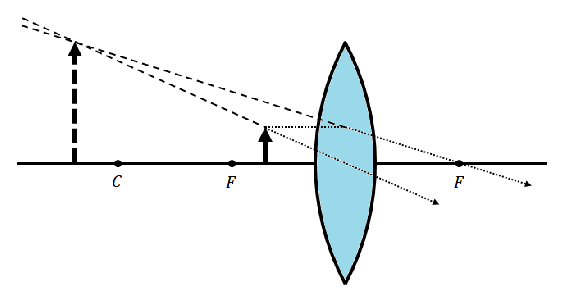
\includegraphics[width=\textwidth]{convex1.eps}
        \caption{\textit{Object between} $P$ \textit{and} $F$.}
        \end{minipage}
        \hfill
        \begin{minipage}[b]{0.49\textwidth}
            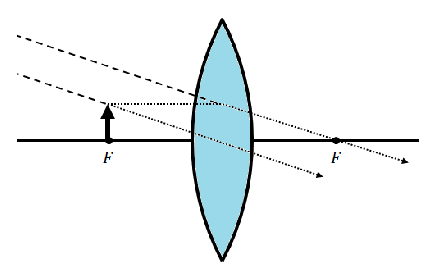
\includegraphics[width=\textwidth]{convex2.eps}
            \caption{\textit{Object on} $F$.}
        \end{minipage}
    \end{figure}
    \begin{figure}[H]
        \centering
        \begin{minipage}[b]{0.49\textwidth}.
        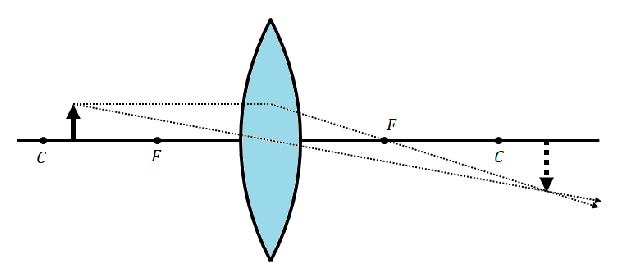
\includegraphics[width=\textwidth]{convex3.eps}
        \caption{\textit{Object between} $F$ \textit{and} $C$.}
        \end{minipage}
        \hfill
        \begin{minipage}[b]{0.49\textwidth}
            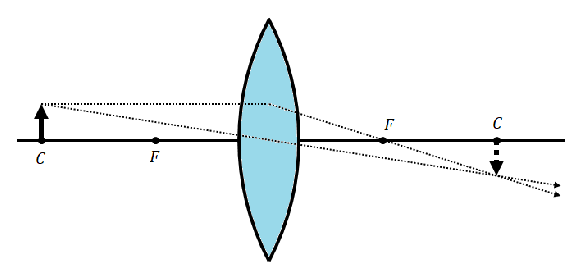
\includegraphics[width=\textwidth]{convex4.eps}
            \caption{\textit{Object on} $C$.}
        \end{minipage}
    \end{figure}
    \begin{figure}[H]
        \centering
        \begin{minipage}[b]{0.49\textwidth}.
        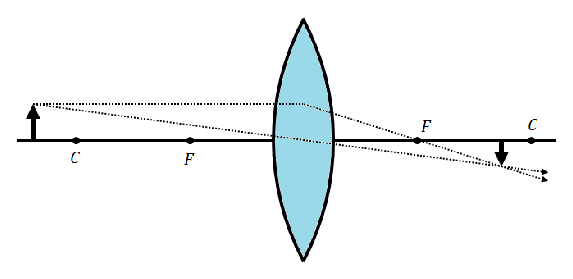
\includegraphics[width=\textwidth]{convex5.eps}
        \caption{\textit{Object beyond} $C$.}
        \end{minipage}
        \hfill
        \begin{minipage}[b]{0.49\textwidth}
            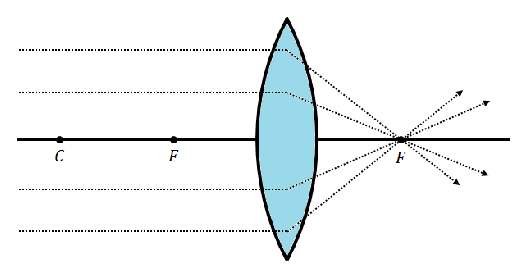
\includegraphics[width=\textwidth]{convex6.eps}
            \caption{\textit{Object at infinity}.}
        \end{minipage}
    \end{figure}
    \quad\textbf{Concave Lens}
    \begin{enumerate}
        \item \textit{Object between} $P$ \textit{and infinity}: if the object is a finite distance away from the mirror, the image formed is between the pole and the focal point, and is virtual (since the reflected rays \textit{produced} intersect), inverted, and smaller than the original object.
        \item \textit{Object at infinity}: if the object is at infinity, then the ``image" formed will be a point at the focal point.
    \end{enumerate}
    \subsection{Physical Optics}
    \quad Super quick history lesson: Newton came out with his Corpuscular Theory, assuming light to be a particle. It explained reflection, refraction, but failed to explain interference, polarization, or diffraction. Huygens then dethroned it with his Wave Theory, assuming light to be a wave; he explained all of the above except for polarization. \textit{This theory is what we will mainly focus on here}. Flash-forward a couple centuries to steam engines, top hats, and the development of E$\&$M. Our old pal Maxwell comes out describing light as an electromagnetic wave (remember $\varepsilon_0\mu_0=c^{-2}$) and he can describe it all...except emmision and absorption of light. He basically could not explain black-body radiation that we studied in Thermodynamics. Max Plank solves the issue by introducing the idea of quantization of light (basically he assumed light waves came in packets), and it was the first \textit{implicit} use of dual nature of light. Enter Albert Einstein, who used Plank's work to develop his Quantum Theory of Light which explained it all from diffraction to the photoelectric effect...except, he could not explain interference, diffraction or polarization. Finally came the modern Dual-Character Theory where we analyze some aspects using wave nature and others using particle nature.
    \newline\quad \textbf{Wavefront}: the set of all points that are in phase in a 2D wave is called a wavefront.
    \begin{enumerate}
        \item Each point source of light is where a wave spread out from in all directions.
        \item Each point on a wave front is the source of smaller disturbances called \textit{secondary wavelets}.
        \item The forward envelope of each secondary wavelet that are in phase will form another primary wavelet as shown in Figure (25).
        \item The wavefront is always perpendicular to the direction of the wave's travel.
    \end{enumerate}
    \begin{figure}[H]
        \centering
        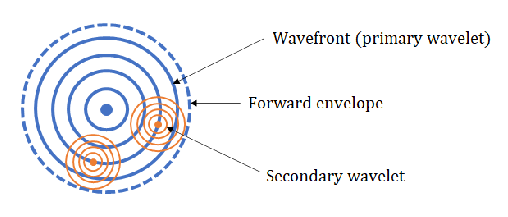
\includegraphics[scale=1.5]{wavefront.eps}
        \caption{This is how a wavefront, like light, expands.}
    \end{figure}
\end{document}